%% Manuscript for submission to Earth Critical Zone (Elsevier)
%% elsarticle Harvard reference style
%% ============================================================

\documentclass[preprint,review,12pt,authoryear]{elsarticle}

\usepackage{amssymb}
\usepackage{amsmath}
\usepackage{booktabs}
\usepackage[utf8]{inputenc}
\usepackage[T1]{fontenc}
\usepackage{graphicx}
\usepackage{lineno}
\usepackage{url}

\journal{Earth Critical Zone}

\begin{document}

\begin{frontmatter}

\title{Parametric identifiability of a multiplicative USLE erodibility correction for hydraulically impeded Plinthosols}

\author[1]{Luiz Diego Vidal Santos\corref{cor1}}
\ead{ldvsantos@uefs.br}
\cortext[cor1]{Corresponding author}

\author[2]{Emersson Guedes da Silva}
\ead{academicoguedes@gmail.com}

\author[3]{Francisco Sandro Rodrigues Holanda}
\ead{fholanda@academico.ufs.br}

\author[3]{Marcos Oliveira Santos}
\ead{marcos.oliveira@academico.ufs.br}

\author[4]{Renisson Neponuceno de Araújo Filho}
\ead{renisson.neponuceno@ufrpe.br}

\author[3]{Henrique Antonio Silva}
\ead{henriqueantoniosilva@hotmail.com}

\author[5]{Jémisson Mattos dos Santos}
\ead{jmsantos4@uesc.br}


\affiliation[1]{organization={Programa de P\'{o}s-Gradua\c{c}\~{a}o em Planejamento Territorial, Universidade Estadual de Feira de Santana},
            city={Feira de Santana},
            postcode={44036-900},
            state={BA},
            country={Brazil}}

\affiliation[2]{organization={Departamento de Zootecnia, Universidade Federal de Sergipe},
            city={S\~{a}o Crist\'{o}v\~{a}o},
            postcode={49100-000},
            state={SE},
            country={Brazil}}

\affiliation[3]{organization={Departamento de Engenharia Agron\^{o}mica, Universidade Federal de Sergipe},
            city={S\~{a}o Crist\'{o}v\~{a}o},
            postcode={49100-000},
            state={SE},
            country={Brazil}}

\affiliation[4]{organization={Departamento de Tecnologia Rural, Universidade Federal Rural de Pernambuco},
            city={Recife},
            postcode={52171-900},
            state={PE},
            country={Brazil}}

\affiliation[5]{organization={Departamento de Ci\^{e}ncias Agr\'{a}rias e Ambientais, Universidade Estadual de Santa Cruz},
            city={Ilh\'{e}us},
            postcode={45662-900},
            state={BA},
            country={Brazil}}

\begin{abstract}
Accelerated water erosion in tropical soils depends on surface and subsurface attributes that control runoff, vegetation cover and linear-feature stability. In Plinthosols, subsurface hydraulic impedance, aluminum phytotoxicity and geotechnical vulnerability may increase effective erodibility beyond the $K$-factor nomograph estimate, whereas existing corrections do not integrate these mechanisms. We evaluated the parametric identifiability and physical consistency of a five-parameter multiplicative correction ($K_{\mathrm{plint}} = K_{\mathrm{RUSLE}} \times \alpha \times \beta \times \gamma$) through five computational tests anchored in measurements from a Haplic Plinthosol (basic infiltration rate of 1.53--3.13~cm/h, aluminum saturation of 15--99\%, six erosion features), virtual Ferralsol and Acrisol profiles, and site comparisons between bare soil and low palisades. Calibration recovered the hydraulic-biological parameters with bias below 15\% under 30\% noise, whereas the geotechnical pair showed equifinality mitigable by stability priors. Sobol analysis indicated dominance of the hydraulic exponent in the Plinthosol (63--78\% of variance), whereas toxicity dominated in the Ferralsol, consistent with the pedological contrast among classes. The multiclass design separated the hydraulic contribution of the Plinthosol, the partial response of the Acrisol and the negative control of the Ferralsol, reducing ambiguity among infiltration, toxicity and slope amplification. Green--Ampt generated a runoff coefficient of 0.56 for the Plinthosol under 60~mm/h and zero runoff in the Ferralsol, consistent with the hydraulic threshold. The exploratory campaign on a 22$^{\circ}$ slope, with bare soil and low palisades ($\sim$20~cm), recorded $CV \approx 80\%$ among replicates and a bare-soil/palisade ratio of 2.34, equivalent to $C \cdot P \approx 0.43$. Site data provided observational noise and empirical cover-management information to parameterize simulations and prioritize hierarchical calibration. The multiplicative structure showed sufficient identifiability to guide instrumented plots under natural rainfall and jointly estimate $K_{\mathrm{plint}}$, cover and management.
\end{abstract}

\begin{highlights}
\item Five-parameter multiplicative correction integrates hydraulic, phytotoxic and geotechnical amplifiers of USLE $K$
\item Sobol analysis shows hydraulic impedance governs 63--78\% of amplification variance in Plinthosols
\item Hydraulic-biological parameters recoverable with $<$15\% bias under 30\% noise
\item Green--Ampt model validates infiltration-rate threshold separating Plinthosol from Ferralsol runoff regimes
\item Geotechnical equifinality confined to shallow features is mitigable by slope-stability priors
\item Field campaign provides observational noise envelope ($CV \approx 80\%$) and $C \cdot P \approx 0.43$ prior for calibration design
\end{highlights}

\begin{keyword}
tropical soil \sep Sobol sensitivity \sep Green--Ampt infiltration \sep aluminum phytotoxicity \sep gully erosion \sep nomograph correction
\end{keyword}

\end{frontmatter}

\linenumbers

%% ================================================================
%%  1. INTRODUCTION
%% ================================================================
\section{Introduction}
\label{sec:intro}

Accelerated water erosion constitutes one of the most severe threats to global agricultural sustainability. Soil loss rates on cultivated land exceed pedogenesis by one to two orders of magnitude across diverse tropical and subtropical regions \citep{montgomery_2007}. Recent estimates indicate that land-use change may amplify global erosion by up to 14\% by 2050 \citep{borrelli_et_al_2017}, whereas erosion-driven degradation already compromises the productive capacity of more than one billion hectares \citep{lal_2001}. The magnitude of the problem makes predictive tools indispensable for conservation planning at both catchment and plot scales.

The Universal Soil Loss Equation and its revised version \citep{wischmeier_smith_1978,renard_et_al_1997} remain the most widely used empirical framework for estimating sheet and rill erosion \citep{alewell_et_al_2019}. The erodibility factor ($K$) synthesizes the intrinsic susceptibility of the soil, yet its estimation via the nomograph of \citet{wischmeier_et_al_1971} depends exclusively on surface-layer attributes such as particle-size distribution, organic matter, structure and permeability \citep{roemkens_et_al_1997}.

This restriction imposes predictive limitations in tropical soils whose oxidic mineralogy generates aggregation patterns distinct from the temperate Mollisols for which the nomograph was developed \citep{alewell_et_al_2019,cassol_et_al_2023}. Field measurements on conservation plots in Brazil show that $K$ estimates frequently diverge by up to one order of magnitude from nomograph predictions \citep{silva_et_al_2009,lafayette_cantalice_coutinho_2011}. In Plinthosols affected by linear erosion features, this discrepancy is amplified by three convergent processes absent from the original formulation. Plinthic horizons with cemented concretions reduce saturated hydraulic conductivity to restrictive levels ($<$\,2~cm/h), inducing profile saturation and surface runoff under moderate rainfall events \citep{wang_et_al_2020,embrapa_2018,horton_1933,bertoni_lombardi_neto_2017}. Subsurface aluminum saturation suppresses root development and reduces vegetation cover \citep{gura_et_al_2022}. Additionally, the evolution from rills to gullies shifts the dominant soil-loss mechanism towards lateral block collapse, headcut retreat and piping \citep{poesen_2018,poesen_et_al_2003,kirkby_bracken_2009,vanmaercke_et_al_2021}. Physically based models capture this erosive continuum \citep{nearing_et_al_1989,sidorchuk_2006}, yet the density of their parameterization limits operational application in data-scarce settings \citep{wilkinson_et_al_2024}.

An alternative that preserves operational applicability consists of correcting the nomograph $K$ via multiplicative factors representing the subsurface processes absent from the original formulation \citep{alewell_et_al_2019}. Models with multiple coupled factors, however, accumulate structural uncertainty; evaluating the sensitivity and identifiability of their parameters before field calibration is therefore indispensable \citep{saltelli_et_al_2004}. Sobol global variance-based analysis quantifies the individual and interactive contribution of each parameter, identifying redundancies and equifinalities that would remain hidden under local approaches \citep{sobol_2001,francois_et_al_2024}.

The Haplic Plinthosol of the Coastal Tablelands of Sergipe, northeastern Brazil, combines low infiltration, high aluminum saturation and shallow to incipient linear features, a combination consistent with hydraulic and chemical restrictions described for Plinthosols and with the morphological evolution of gullies in tropical soils \citep{nascimento_pedrotti_2004,embrapa_2018,gura_et_al_2022,poesen_2018}. This gradient represents a set of amplifiers not accounted for by the $K$ nomograph, whose formulation is based on surface attributes of texture, organic matter, structure and permeability \citep{wischmeier_et_al_1971,roemkens_et_al_1997,alewell_et_al_2019}. The proposed multiplicative correction translates this contrast by applying independent terms to $K_{\mathrm{RUSLE}}$ for hydraulic impedance, phytotoxic penalization and geotechnical vulnerability normalized by $H/H_c$.

Because direct calibration of multivariate models requires prolonged monitoring and high instrumental density \citep{alewell_et_al_2019}, prior computational verification of parametric identifiability, sensitivity and physical consistency reduces the risk of equifinality before experimental investment \citep{saltelli_et_al_2004,beven_freer_2001,her_chaubey_2015}.

The available literature supports isolated components of this problem, because saturated hydraulic conductivity has recently been incorporated as a direct modifier of $K$ at a global scale \citep{gupta_et_al_2024}, (R)USLE reviews have recognized structural limitations in tropical soils and gully studies have described the geomorphological and geotechnical control of linear erosion \citep{benavidez_et_al_2018,alewell_et_al_2019,poesen_2018,vanmaercke_et_al_2021}. This convergence leaves open the test of an integrated formulation that couples subsurface hydraulic impedance, phytotoxic penalization and geotechnical vulnerability of Plinthosols before field calibration.

The proposed formulation is evaluated under the expectation that subsurface hydraulic impedance governs the largest share of amplification variance in the Plinthosol \citep{gupta_et_al_2024}. We further expect that the parameters translating hydraulic penalization and edaphic toxicity are recoverable with reduced bias under high observational noise \citep{cheviron_et_al_2010,rao_et_al_2016}, whereas the geotechnical parameters may exhibit equifinality confined to the shallow normalized-depth range of the mapped features \citep{gudino_elizondo_et_al_2018}. The Ferralsol, combining favorable drainage, low toxicity and oxide-promoted aggregate stability \citep{barthes_roose_2002}, should operate as a reference of $\delta \approx 1$, enabling isolation of each amplifying effect during calibration.

This study evaluates the mathematical identifiability and physical consistency of a multiplicative correction factor that translates these three mechanisms as independent amplifiers of $K$, with five free parameters. The evaluation combines five computational tests anchored in measurements at the Haplic Plinthosol experimental site in the Coastal Tablelands of Sergipe, an exploratory campaign on an adjacent slope comparing bare soil and low palisades, and virtual Ferralsol and Acrisol profiles parameterized from the regional literature \citep{silva_et_al_2009,bertoni_lombardi_neto_2017}.

%% ================================================================
%%  2. MODEL FORMULATION
%% ================================================================
\section{Formulation of the $K_{\mathrm{plint}}$ model}
\label{sec:model}

\subsection{Conceptual justification and multiplicative structure}

As noted above, the $K$ nomograph does not incorporate subsurface processes that, in tropical Plinthosols, amplify soil loss beyond the prediction of $K_{\mathrm{RUSLE}}$. The ratio between observed and estimated erodibility ($\delta = K_{\mathrm{obs}}/K_{\mathrm{RUSLE}}$) may exceed unity when hydraulic impedance, aluminum toxicity and geotechnical vulnerability converge in the same profile \citep{poesen_2018}.

The proposed formulation translates these three mechanisms as independent multiplicative factors applied to $K_{\mathrm{RUSLE}}$ (Eq.~\ref{eq:kplint}).

\begin{equation}
K_{\mathrm{plint}} = K_{\mathrm{RUSLE}} \times \alpha(\mathrm{BIR}) \times \beta(m_{\mathrm{Al}}) \times \gamma\!\left(\frac{H}{H_c}\right)
\label{eq:kplint}
\end{equation}

The multiplicative structure implies that each factor operates as an independent amplifier. When none of the three amplifying conditions is present (well-drained soil, no aluminum toxicity, no deep erosion feature), all three factors equal unity and $K_{\mathrm{plint}}$ reduces to $K_{\mathrm{RUSLE}}$.

Conversely, when all three conditions converge, as in Plinthosols with active gullies, the factors multiply and $\delta$ may reach values of 2--10 or higher. The ratio $\delta = \alpha \times \beta \times \gamma$ is dimensionless and independent of the absolute value of $K_{\mathrm{RUSLE}}$, allowing comparison of amplification across pedological classes with different basal erodibility.

\subsection{Hydraulic amplification factor ($\alpha$)}

In soils with good internal drainage, most precipitation infiltrates and percolates vertically, generating minimal surface runoff and thus limited energy for particle detachment and transport \citep{deroo_1992}. In Plinthosols, subsurface horizons with plinthite or petroplinthite exhibit saturated hydraulic conductivity far below that of the overlying horizons \citep{de_moraes_et_al_2006}.

This contrast creates a barrier to percolation that favors profile saturation and infiltration-excess (effective Hortonian) runoff \citep{padmanabhan_2005}. The basic infiltration rate (BIR), measured in the field by double-ring infiltrometer, reflects this integrated impedance and constitutes the most accessible input for expressing the hydrological contrast among soil classes \citep{bertoni_lombardi_neto_2017}.

The factor $\alpha$ penalizes soils whose BIR falls below a reference threshold $\mathrm{BIR_{ref}}$ = 6.0~cm/h, below which the profile predominantly operates under concentrated-flow regime (Eq.~\ref{eq:alpha}).

\begin{equation}
\alpha(\mathrm{BIR}) = \left(\frac{\mathrm{BIR_{ref}}}{\mathrm{BIR_{local}}}\right)^{n_1}, \quad \mathrm{BIR_{local}} < \mathrm{BIR_{ref}}; \quad \alpha = 1 \text{ otherwise}
\label{eq:alpha}
\end{equation}

The smaller the infiltration rate relative to the threshold, the greater the fraction of precipitation converted to runoff and, consequently, the greater the effective erosive energy incident on the surface \citep{kinnell_2005}. The exponent $n_1$ governs the intensity of this penalization as BIR decreases.

For $n_1 = 1$ the relationship is linear, so that halving BIR doubles $\alpha$. Values of $n_1 > 1$ produce more severe penalization in very impermeable soils, whereas $n_1 < 1$ attenuates the differentiation between soils with moderate and very low BIR. The threshold $\mathrm{BIR_{ref}}$ = 6.0~cm/h corresponds to the lower limit of soils classified as well-drained in the tropical literature and was adopted as the neutrality point ($\alpha = 1$) of the hydraulic factor \citep{embrapa_2018}.

\subsection{Edaphic toxicity penalization factor ($\beta$)}

Aluminum saturation ($m_{\mathrm{Al}}$) constitutes an edaphic phytotoxicity indicator, and horizons with $m_{\mathrm{Al}}$ exceeding 50\% are classified as alic, with severe restriction on root development \citep{embrapa_2018}. In degraded pastures on Plinthosols, subsurface toxicity may progressively suppress vegetation cover and reduce soil protection against raindrop impact and concentrated flow, establishing an indirect mechanism of soil-loss amplification that operates via biological pathways (root and canopy suppression) rather than exclusively via hydraulic or geotechnical pathways \citep{kochian_et_al_2005,gyssels_et_al_2005}.

The factor $\beta$ translates this mechanism via a sigmoid function with an activation threshold (Eq.~\ref{eq:beta}).

\begin{equation}
\beta(m) = 1 + \frac{\beta_{\max} - 1}{1 + \exp\!\left[-k_2\,(m - m_0)\right]}
\label{eq:beta}
\end{equation}

The inflection point $m_0 = 50\%$ coincides with the conventional alic character threshold and defines the aluminum saturation at which the toxicity effect reaches half its maximum intensity. For $m_{\mathrm{Al}}$ well below 50\% the denominator is large and $\beta$ approaches~1, indicating that the toxicity is insufficient to measurably suppress vegetation.

For $m_{\mathrm{Al}}$ well above 50\% the function converges to $\beta_{\max}$, representing the maximum amplification attributable solely to toxicity. The parameter $k_2$ controls the steepness of the transition, with high values producing an abrupt transition around 50\% and low values yielding a smooth gradient across the full saturation range.

\subsection{Geotechnical vulnerability factor ($\gamma$)}

The third mechanism is exclusive to erosion features with depth sufficient to mobilize soil volumes by bank failure, a process absent in sheet erosion or shallow rills. Gullies develop vertical or sub-vertical walls whose stability depends on the equilibrium between self-weight-induced shear stress and the shear strength at the failure surface \citep{fredlund_rahardjo_1993}. The critical vertical-cut height ($H_c$) is the depth above which collapse becomes mechanically inevitable, and the ratio $H/H_c$ expresses the proximity of a feature to this threshold in normalized terms (0 = no feature, 1 = imminent collapse).

The factor $\gamma$ assumes unity when $H/H_c = 0$ (soil without erosion feature) and increases with feature depth according to a power expansion (Eq.~\ref{eq:gamma}).

\begin{equation}
\gamma\!\left(\frac{H}{H_c}\right) = 1 + k_3 \cdot \left(\frac{H}{H_c}\right)^{n_3}
\label{eq:gamma}
\end{equation}

The parameter $k_3$ scales the magnitude of geotechnical amplification and $n_3$ governs the curvature of the response. High values of $n_3$ ($>$\,2) cause $\gamma$ to remain near~1 for shallow features and rise abruptly only as $H/H_c$ approaches~1, a physically coherent behavior because the soil volume mobilized by failure wedge grows with cubic or higher power of the wall height.

The critical height $H_c$ is calculated from Rankine earth-pressure theory for vertical cuts.

\begin{equation}
H_c = \frac{2c}{\gamma_{\mathrm{sat}}} \cdot \tan\!\left(45^\circ + \frac{\phi}{2}\right) + \frac{2c}{\gamma_{\mathrm{sat}} \cdot \tan\!\left(45^\circ + \frac{\phi}{2}\right)}
\label{eq:hc}
\end{equation}

\noindent where $c$ is the effective cohesion (kPa), $\phi$ the internal friction angle ($^\circ$) and $\gamma_{\mathrm{sat}}$ the saturated unit weight (kN/m$^3$). Increasing values of $H/H_c$ increase the geotechnical contribution only as the feature approaches the critical threshold, preserving $\gamma \approx 1$ in shallow rills and allowing progressive amplification in deep gullies.

\subsection{Free and fixed parameters}

The model has five free parameters ($n_1$, $\beta_{\max}$, $k_2$, $k_3$ and $n_3$) to be estimated by field calibration, and two a-priori-fixed parameters ($\mathrm{BIR_{ref}} = 6$~cm/h and $m_0 = 50\%$) derived from pedological evidence and phytotoxicity thresholds documented in tropical soils \citep{embrapa_2018}. The ratio $\delta = K_{\mathrm{plint}} / K_{\mathrm{RUSLE}} = \alpha \times \beta \times \gamma$ synthesizes the total erodibility amplification and constitutes the response variable of the five computational tests described in Section~\ref{sec:validation}.

%% ================================================================
%%  3. COMPUTATIONAL VALIDATION STRATEGY
%% ================================================================
\section{Computational validation strategy}
\label{sec:validation}

\subsection{Study area and input data}

The experimental site is located in the Coastal Tablelands geomorphological unit of the state of Sergipe, northeastern Brazil, on a Haplic Plinthosol developed from sediments of the Barreiras Group \citep{nascimento_pedrotti_2004}. The climate is tropical humid (As in the K\"{o}ppen classification), with mean annual precipitation of 1200--1400~mm concentrated between April and August and mean temperature of 25~$^\circ$C.

The predominant land use is degraded pasture with sparse cover, a condition that exposes the subsurface horizons to direct action of concentrated flow. The site occupies a gently undulating interfluve where the combination of sparse vegetation and subsurface plinthite has favored the development of multiple linear erosion features along the drainage axis (Fig.~\ref{fig:area}a).

Six active erosion features (F1--F6) were identified from UAV-derived orthomosaics with a mean point-cloud density of 120~points/m$^2$ and their morphometric parameters (depth, width and length) validated by direct field measurements with measuring tape (Fig.~\ref{fig:area}b--c). Feature depths ranged from 0.40~m (F2) to 1.50~m (F5), corresponding to normalized depths $H/H_c$ of 0.12--0.45 relative to the critical height $H_c = 3.35$~m calculated from field-measured geotechnical parameters via Eq.~\ref{eq:hc}.

\begin{figure}[htbp]
\centering
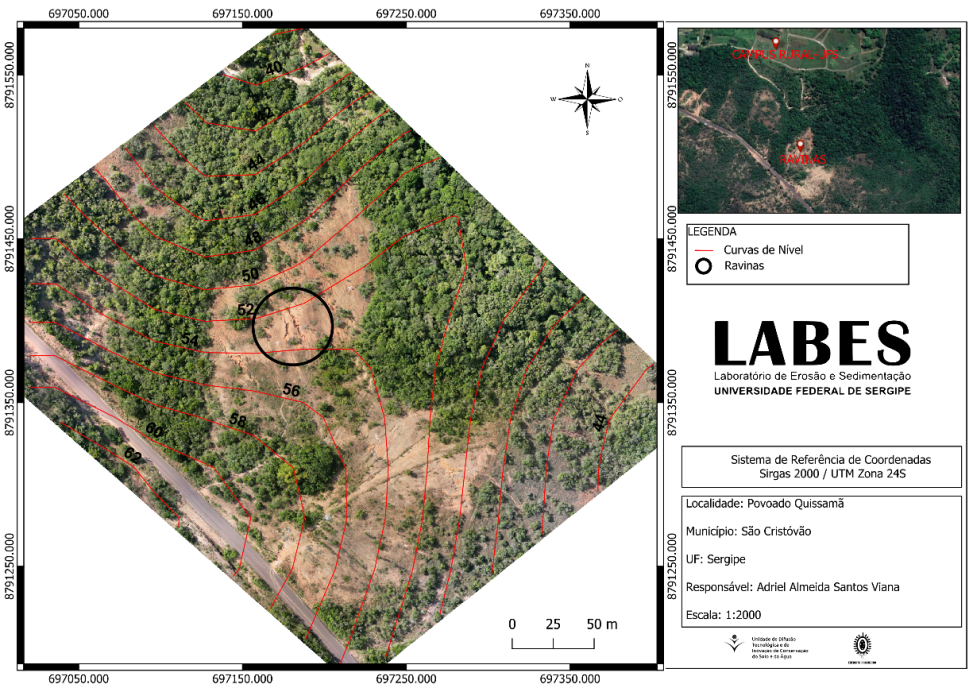
\includegraphics[width=0.85\textwidth]{fig_00a_area_estudo_aerea.png}\\[6pt]
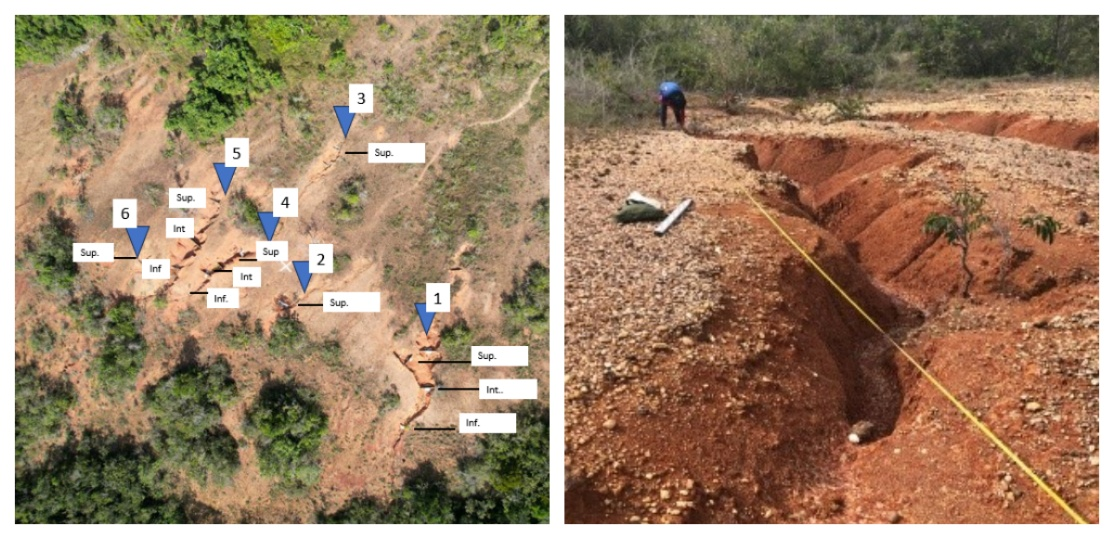
\includegraphics[width=0.85\textwidth]{fig_00b_feicoes_drone_campo.jpeg}
\caption{Experimental site on the Coastal Tablelands of Sergipe, northeastern Brazil. (a)~Aerial view showing the degraded-pasture landscape and the occurrence of linear erosion features on the Haplic Plinthosol (map lines delineate the study area and do not necessarily depict accepted national boundaries). (b)~UAV-derived orthomosaic showing the spatial distribution of the mapped erosion features. (c)~Field measurement of morphometric parameters (depth, width and length) in one of the active erosion features.}
\label{fig:area}
\end{figure}

All input properties of the Plinthosol were obtained from field measurements and laboratory analyses conducted on samples collected at the experimental site. The basic infiltration rate (BIR) was determined in situ by double-ring infiltrometer tests on three representative horizons (Ap, BAc and Bf), yielding values of 3.13, 1.53 and 1.59~cm/h, respectively, which confirm that the plinthic and sub-plinthic horizons impose hydraulic impedance well below the adopted reference threshold ($\mathrm{BIR_{ref}} = 6.0$~cm/h).

Aluminum saturation ($m_{\mathrm{Al}}$) was quantified by routine soil-fertility analysis of samples from each genetic horizon, with values ranging from 15.2\% in the Ap to 99.2\% in the Bf, a vertical gradient consistent with progressive base leaching and exchangeable-aluminum concentration at depth.

Geotechnical parameters (effective cohesion $c = 13.02$~kPa, internal friction angle $\phi = 34.93^\circ$ and saturated unit weight $\gamma_{\mathrm{sat}} = 19.93$~kN/m$^3$) were determined by direct-shear testing (ASTM D3080) on undisturbed samples extracted from the Bt horizon under saturated conditions.

The erodibility $K_{\mathrm{RUSLE}} = 0.035$~t\,h\,MJ$^{-1}$\,mm$^{-1}$ was estimated from the particle-size distribution, organic-matter content, structure code and permeability class of the surface horizon using the standard nomograph \citep{wischmeier_et_al_1971}. These field-derived values constitute the primary input dataset for all five computational tests (Table~\ref{tab:profiles}, column ``Plinthosol (field)'').

Two virtual profiles (Ferralsol and Acrisol) were parameterized from median values in the regional literature for BIR, aluminum saturation, geotechnical properties and $K_{\mathrm{RUSLE}}$ \citep{silva_et_al_2009,bertoni_lombardi_neto_2017}. The Ferralsol operates as a negative control ($\alpha \approx \beta \approx \gamma \approx 1$), representing well-drained soils without hydraulic impedance, toxicity or deep erosion features, while the Acrisol functions as a partial control, sharing moderate hydraulic impedance in the Bt horizon but without plinthite or extreme aluminum toxicity. No field measurements were conducted on these two classes; their role is exclusively computational, serving as benchmarks against which the Plinthosol amplification is evaluated.

\begin{table}[htbp]
\centering
\caption{Properties of the three soil profiles used in the simulations. Plinthosol values were obtained from field measurements.}
\label{tab:profiles}
\small
\begin{tabular}{@{}l r r r@{}}
\toprule
Property & Plinthosol (field) & Ferralsol (virtual) & Acrisol (virtual) \\
\midrule
BIR upper (cm/h) & 3.13 & 12.0 & 4.5 \\
BIR intermediate (cm/h) & 1.53 & 9.0 & 2.5 \\
BIR lower (cm/h) & 1.59 & 7.0 & 2.8 \\
$K_{\mathrm{sat,eff}}$ (cm/h) & 0.50 & 8.0 & 1.0 \\
$m_{\mathrm{Al}}$ Ap (\%) & 15.2 & 10.0 & 20.0 \\
$m_{\mathrm{Al}}$ subsurface (\%) & 84--99 & 20.0 & 45.0 \\
$c$ (kPa, saturated) & 13.02 & 30.0 & 18.0 \\
$\phi$ ($^\circ$) & 34.93 & 30.0 & 32.0 \\
$\gamma_{\mathrm{sat}}$ (kN/m$^3$) & 19.93 & 18.0 & 19.0 \\
$H_c$ (m) & 3.35 & 5.77$^a$ & 4.33$^a$ \\
$H/H_c$ mean & 0.28 & 0.00 & 0.08 \\
$K_{\mathrm{RUSLE}}$ (t\,h\,MJ$^{-1}$\,mm$^{-1}$) & 0.035 & 0.015 & 0.025 \\
\bottomrule
\end{tabular}

\noindent $^a$ Calculated from Eq.~\ref{eq:hc}.
\end{table}

\subsection{Exploratory slope campaign with low stone palisades}
\label{sec:field-palisades}

The exploratory campaign was installed on a Plinthosol slope adjacent to the target site, under degraded pasture and with a slope angle of 22$^\circ$. The setup used nine reduced ramps of 2.40~m $\times$ 0.50~m, each with an area of 1.20~m$^2$, of which seven remained under bare soil and two received low stone palisades, with approximately 20~cm of granular fragments placed transverse to flow.

Sediment-collection tubes were positioned at the base of the ramps to retain sediment mobilized by natural rainfall, whereas the undisturbed block extracted from the slope provided the direct-shear parameters used to estimate $H_c$ (Fig.~\ref{fig:sitio}). This setup was designed to estimate the observational-noise envelope and a cover-management prior for subsequent calibrations of $K_{\mathrm{plint}} \cdot C \cdot P$.

\begin{figure}[htbp]
\centering
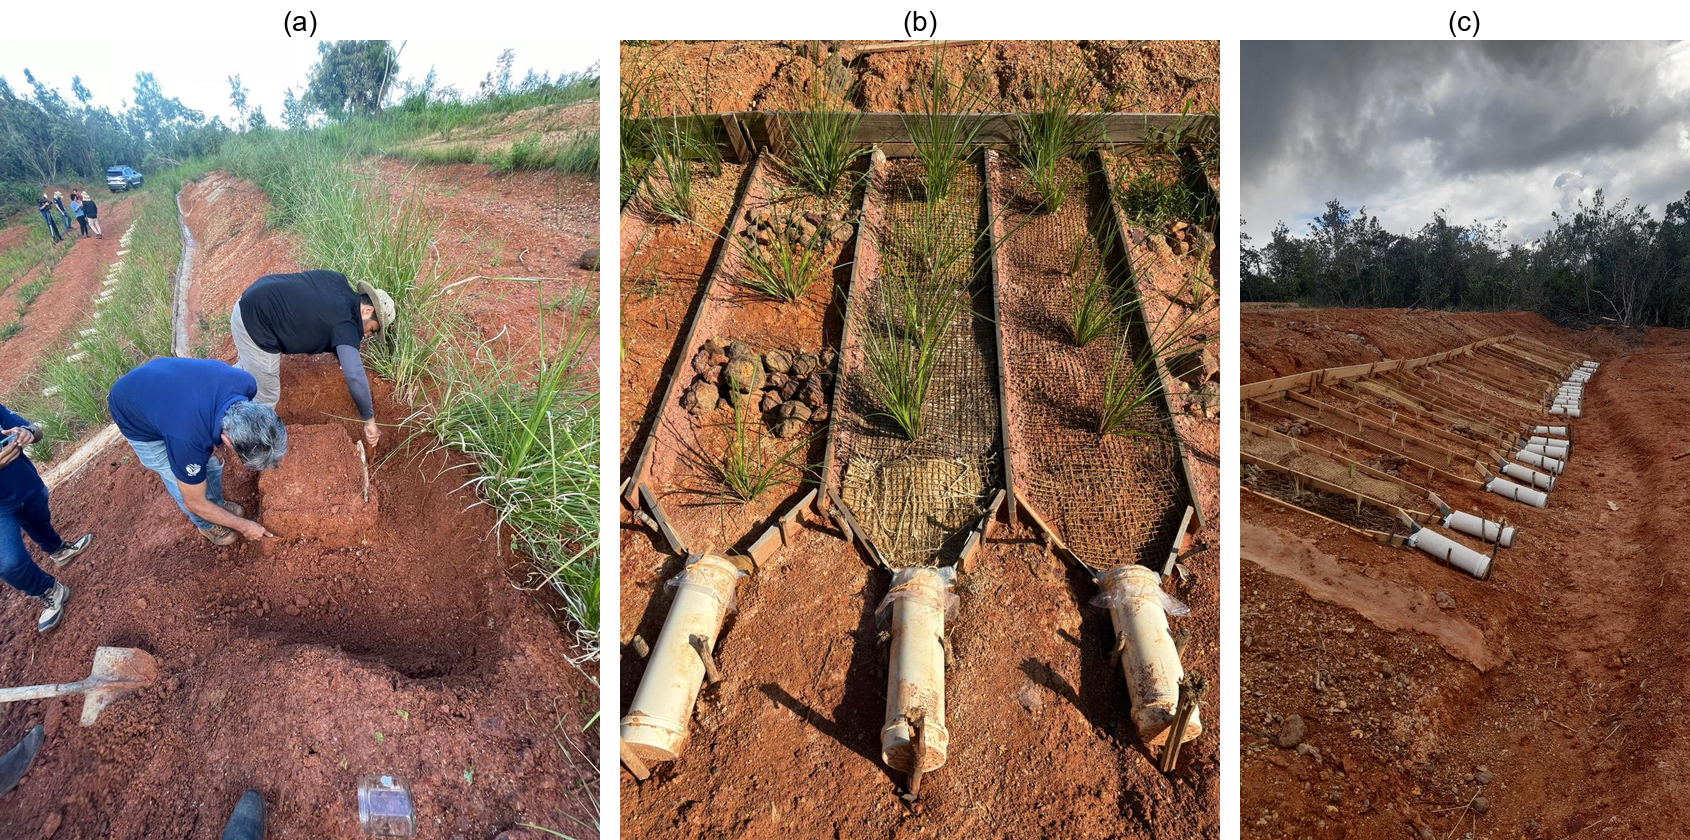
\includegraphics[width=\textwidth]{fig_09_sitio_experimental.png}
\caption{Exploratory slope setup on Plinthosol used to compare bare soil and low stone palisades. (a)~Undisturbed block extracted for direct-shear testing. (b)~Sediment-collection tubes positioned at the base of the reduced ramps. (c)~Slope with bare-soil plots and low stone palisades.}
\label{fig:sitio}
\end{figure}

\subsection{Target parameters for synthetic calibration}

For tests requiring known ``true'' values, the following were adopted: $n_1 = 1.0$, $\beta_{\max} = 2.5$, $k_2 = 0.10$, $k_3 = 3.0$, $n_3 = 2.0$. These values were chosen within physically plausible ranges, without claiming to represent the actual site parameters (which will only be known after field calibration).

\subsection{Test~1: Synthetic calibration (parameter recovery)}

The objective is to verify whether the proposed four-step sequential calibration protocol recovers the five known parameters from noisy data. Synthetic $\delta_{\mathrm{obs}}$ was generated for 42 virtual plots (16 Plinthosol, 12 Ferralsol, 14 Acrisol) by multiplying $\delta_{\mathrm{true}}$ by multiplicative Gaussian noise with CV of 10--30\%, so that $\delta_{\mathrm{obs}} = \delta_{\mathrm{true}} \times (1 + \varepsilon)$ with $\varepsilon \sim N(0, \mathrm{CV}^2)$, truncated at $\delta_{\mathrm{obs}} > 0$ for physical admissibility (no realization violated this constraint in the 30 replicates). The calibration protocol follows the field sequence: negative-control verification ($\delta_{\mathrm{Lat}} \approx 1$), marginal estimation of $\alpha$ via the Acrisol, calibration of $\beta$ via the Plinthosol horizon contrast, and calibration of $\gamma$ via the geotechnical residual, followed by simultaneous optimization via Levenberg--Marquardt. Each CV level was replicated 30 times.

\subsection{Test~2: Global sensitivity analysis (Sobol)}

First-order ($S_1$) and total ($S_T$) Sobol indices \citep{sobol_2001} were calculated to quantify each parameter's contribution to the variance of $\delta$ in four representative scenarios: Plinthosol intermediate (BIR = 1.53, $m = 84\%$, $H/H_c = 0.33$), Plinthosol upper (BIR = 3.13, $m = 15\%$, $H/H_c = 0.12$), Acrisol (BIR = 2.5, $m = 45\%$, $H/H_c = 0.08$) and Ferralsol (BIR = 9.0, $m = 20\%$, $H/H_c = 0$). Saltelli sampling \citep{saltelli_et_al_2004} with $N = 1024$ generated 12\,288 model evaluations. The five parameters were sampled as independent uniform variables, a premise supported by the multiplicative formulation in which $\alpha$, $\beta$ and $\gamma$ represent physically distinct mechanisms without a-priori parametric correlation. Parameter bounds were $n_1 \in [0.1, 3.0]$, $\beta_{\max} \in [1.1, 5.0]$, $k_2 \in [0.01, 0.50]$, $k_3 \in [0.5, 10.0]$ and $n_3 \in [1.0, 4.0]$.

\subsection{Test~3: Slope stability and $\gamma$ validation}
\label{sec:test3}

The Rankine factor of safety (FS) \citep{rankine_1857} for vertical cuts was calculated for $H/H_c$ from 0.05 to 0.95 under six levels of relative pore pressure ($r_u = 0$ to 0.5), using the field geotechnical parameters of the Plinthosol. The volume mobilized by a planar failure wedge was normalized and modeled as a geotechnical contribution proxy ($\delta_{\mathrm{geo}} \propto V_{\mathrm{norm}}/\mathrm{FS}$). The function $\gamma = 1 + k_3(H/H_c)^{n_3}$ was fitted to the proxy by non-linear least squares, and the FS corresponding to each of the six real features (F1--F6) was verified.

\subsection{Test~4: Infiltration and runoff generation (Green--Ampt)}

A Green--Ampt infiltration model \citep{green_ampt_1911} was applied to the three soil profiles under rainfall events with $I_{30}$ of 5--100~mm/h and duration of 60~min. The effective $K_{\mathrm{sat}}$ of each profile corresponds to the limiting horizon (minimum across layers). The runoff coefficient (RC) was calculated and the ratio $\mathrm{RC}_{\mathrm{soil}}/\mathrm{RC}_{\mathrm{Ferralsol}}$ compared with $\alpha(\mathrm{BIR})$ for different values of $n_1$, evaluating the consistency between the analytical hydraulic model and the proposed functional form.

\subsection{Test~5: Virtual erosion (simplified WEPP-type model)}

The runoff generated by the Green--Ampt model was converted to bed shear stress ($\tau = \rho g h S$, uniform flow (Manning's equation)) and to soil loss via a detachment model ($D = k_r(\tau - \tau_c)$ for $\tau > \tau_c$). The erodibility $K_{\mathrm{obs}}$ was inverted via the USLE relationship ($K_{\mathrm{obs}} = A/(EI_{30} \times LS)$) and the discrepancy $\delta_{\mathrm{obs}} = K_{\mathrm{obs}}/K_{\mathrm{RUSLE}}$ compared with $\delta_{\mathrm{mod}}$ predicted by Eq.~\ref{eq:kplint} using the target parameters of Section~3.2. Intrinsic erodibility parameters ($k_r$, $\tau_c$) were estimated from the literature for tropical soils.

%% ================================================================
%%  4. RESULTS AND DISCUSSION
%% ================================================================
\section{Results and discussion}
\label{sec:results}

\subsection{Field response of the model factors}

The Sergipe Plinthosol (Table~\ref{tab:profiles}) and the six erosion features mapped in the field (Fig.~\ref{fig:area}b--c) provide the three directly measurable pedological attributes that parameterize $K_{\mathrm{plint}}$, dispensing with intermediate detailed hydrological modeling.

The BIR of the BAc horizon, 1.53~cm/h, yields $\alpha = (6.0/1.53)^{n_1} = 3.92^{n_1}$. For $n_1 = 1$, the subsurface impedance amplifies effective erodibility by nearly four times relative to a soil at the reference BIR, a magnitude on the same order as the systematic error the original nomograph commits in tropical soils with limiting horizons \citep{alewell_et_al_2019}. In a typical Red-Yellow Ferralsol with BIR of 9~cm/h, $\alpha = 1$ because $\mathrm{BIR} > \mathrm{BIR_{ref}}$, and the same equation operates as a negative control in well-drained soils without additional reparameterization. The hydrological consistency of this contrast is taken up in Test~4.

The phytotoxic factor displays a pronounced vertical gradient. The Ap horizon, with $m_{\mathrm{Al}} = 15.2\%$, yields $\beta \approx 1.04$ for $\beta_{\max} = 2.5$ and $k_2 = 0.10$, practically no amplification. The BAc horizon, in contrast, reaches $m_{\mathrm{Al}} = 99.2\%$ and $\beta \approx 2.47$, near the maximum. The surface may still sustain sparse cover, while horizons exposed at gully banks remain essentially without root protection against detachment by concentrated flow \citep{vannoppen_2015}, a condition that classical RUSLE only indirectly approximates through the $C$ factor.

The geotechnical parameters measured ($c = 13.02$~kPa, $\phi = 34.93^\circ$, $\gamma_{\mathrm{sat}} = 19.93$~kN/m$^3$) yield $H_c = 3.35$~m. The six features have depths of 0.40--1.50~m, corresponding to $H/H_c = 0.12$--0.45, an interval in which $\gamma$ remains near~1 and geotechnical collapse is not yet the dominant soil-loss mechanism. In regional gullies with depth exceeding 2~m ($H/H_c > 0.6$), $\gamma$ may contribute substantially to total amplification, justifying the inclusion of this term in the extended RUSLE. Verification of the factor of safety per feature and the fitting of $\gamma$ are addressed in Test~3.

\subsection{Parameter recovery (Test~1)}

The three hydraulic-biological parameters ($n_1$, $\beta_{\max}$, $k_2$) were recovered by the sequential protocol with median relative bias below 15\% for all synthetic noise levels tested (Fig.~\ref{fig:calibracao}), a necessary condition for $K_{\mathrm{plint}}$ to operate as an extended RUSLE factor on field data with realistic noise. Precision decreased in the order $n_1 > k_2 > \beta_{\max}$ under CV of 30\%, and the higher accuracy of $n_1$ (median 1.01--1.18 versus 1.0) is coherent with the dominance of the hydraulic term in the variance of $\delta$ in the Plinthosol, with direct implications for soil loss predicted by the corrected RUSLE because residual errors in this exponent propagate multiplicatively to the final estimate.

The maximum toxicity amplification ($\beta_{\max} = 2.28$--2.85, true 2.5) and the transition rate ($k_2 = 0.11$--0.13, true 0.10) exhibited comparable biases. The narrow range of $m_{\mathrm{Al}}$ in the exposed horizons attenuates the propagation of these biases to $K_{\mathrm{plint}}$, although the dispersion of $\beta_{\max}$ increased with noise level without generating a systematic trend.

\begin{figure}[htbp]
\centering
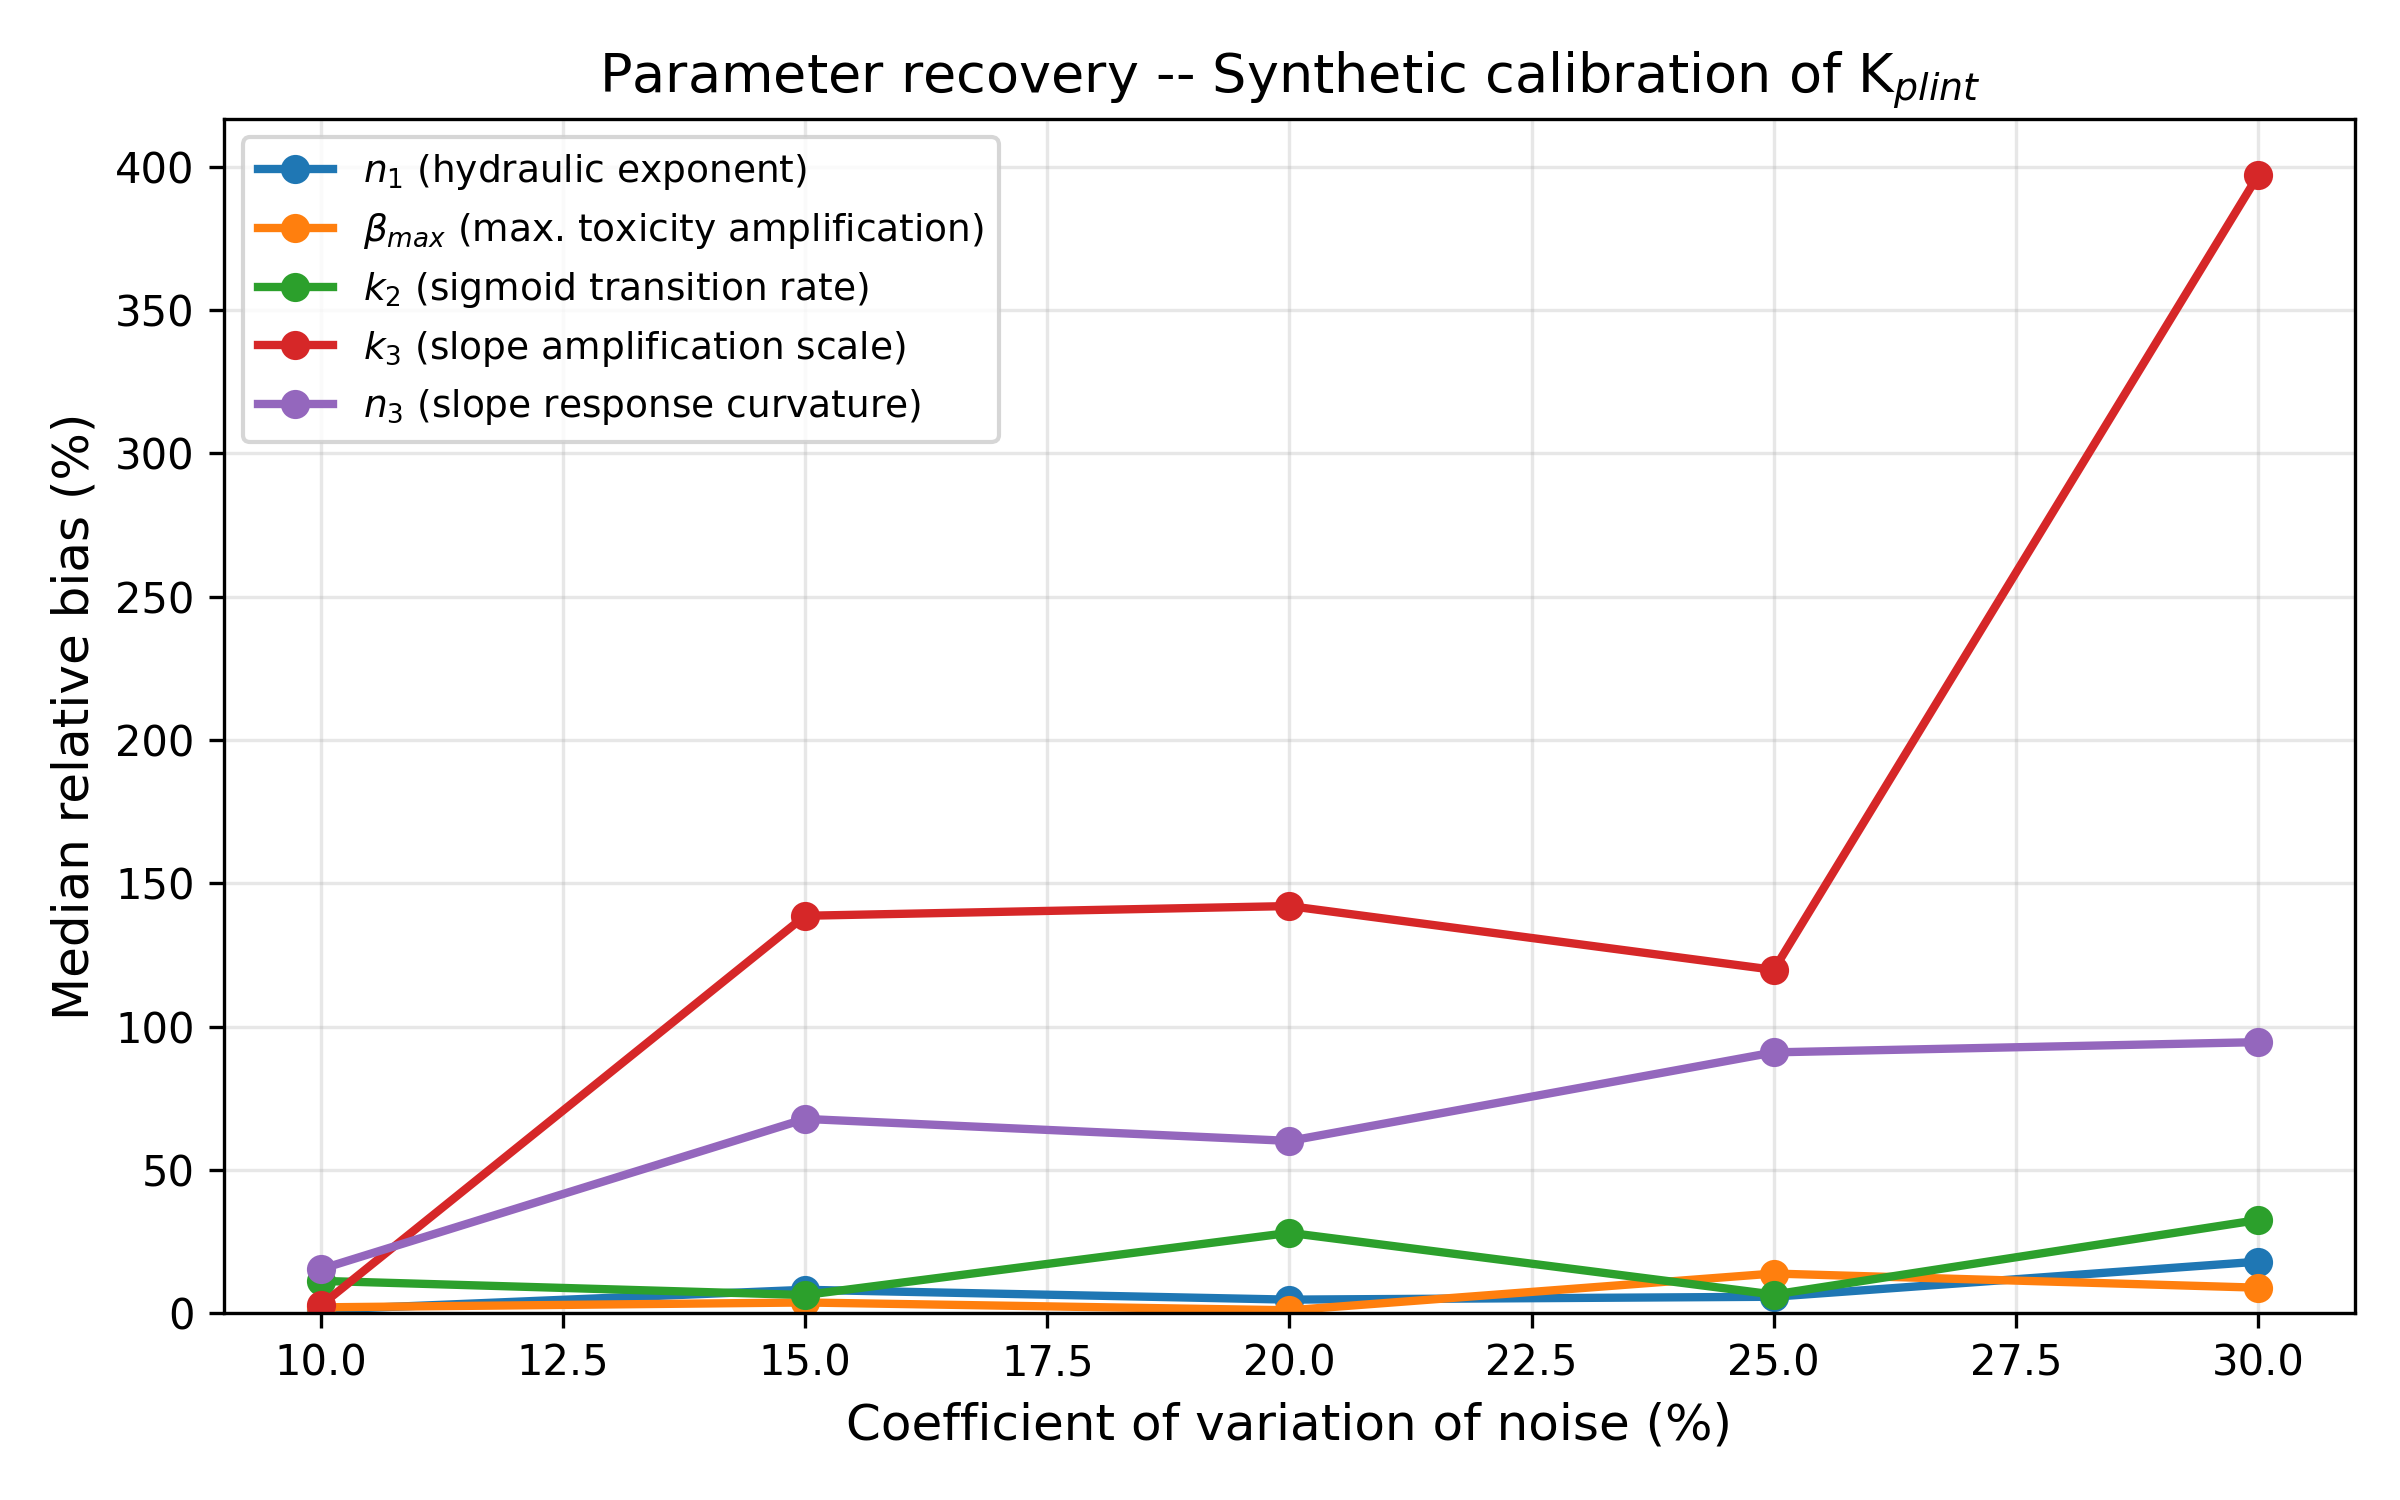
\includegraphics[width=0.9\textwidth]{fig_01_calibracao_sintetica.png}
\caption{Median relative bias of estimated parameters as a function of the coefficient of variation (CV) of synthetic noise.}
\label{fig:calibracao}
\end{figure}

The parameters $k_3$ and $n_3$ exhibited high dispersion and a tendency to converge at the upper bounds of the search ranges (Fig.~\ref{fig:boxplot}), with medians of 14.9 and 3.9 respectively for CV = 30\% (true values 3.0 and 2.0). For $H/H_c = 0.12$--0.45, the product $k_3 \times (H/H_c)^{n_3}$ admits multiple combinations with $\gamma$ near~1.0, generating equifinality. The phenomenon is analogous to that described by \citet{beven_freer_2001} for mechanistic hydrological models and was formalized by \citet{beven_2006} as an intrinsic property of over-parameterized models.

For the operational RUSLE user, this equifinality means that the $\gamma$ term cannot be calibrated using shallow features alone and that estimates in deep gullies must rely on geotechnical priors. \citet{her_chaubey_2015} showed that equifinality tends to diminish when data cover the model's dynamic range, suggesting that features with $H/H_c > 0.45$ must be monitored to reduce the indeterminacy of $k_3$ and $n_3$. A Bayesian framework with informative priors derived from the Rankine analysis (Supplementary Material~S1) can constrain the posterior distribution and mitigate the equifinality identified here.

Since the field data from the Plinthosol lack features with $H/H_c > 0.45$, calibration of this factor requires monitoring of features with depth exceeding 1.5~m or complementary geotechnical modeling. This restriction does not invalidate the use of the $K_{\mathrm{plint}}$ structure within RUSLE but delimits the depth range over which the $\gamma$ term can be considered fitted.

\begin{figure}[htbp]
\centering

\includegraphics[width=\textwidth]{fig_02_boxplot_parametros.png}
\caption{Distribution of estimated parameters across 30 replicates per noise level. Red dashed lines indicate true values.}
\label{fig:boxplot}
\end{figure}

The negative control (Ferralsol) yielded median $\delta_{\mathrm{Lat}}$ of 1.04--1.07 across all CV levels, confirming that the model correctly predicts $\delta \approx 1$ when the three amplifying conditions are absent. This behavior follows from the multiplicative formulation, in which $\alpha = 1$ for $\mathrm{BIR} \geq \mathrm{BIR_{ref}}$, $\beta \approx 1$ for $m_{\mathrm{Al}} < 50\%$ and $\gamma = 1$ for $H/H_c = 0$, so that residual noise in $\delta$ is attributable solely to numerical propagation.

The proximity to unity reinforces the pedological specificity of the correction factor and is coherent with the finding that deep Ferralsols tend to exhibit erodibility near or below the nomograph estimate, owing to stable macroaggregation by iron and aluminum oxides \citep{cassol_et_al_2023}. The asymmetry of nomograph error across pedological classes reinforces that $K_{\mathrm{plint}}$ acts in both directions of classical RUSLE: \citet{auerswald_et_al_2014} demonstrated overestimation in soils with stable aggregates and high conductivity, a typical Ferralsol condition, while \citet{ostovari_et_al_2016} observed underestimation in calcareous soils with subsurface impedance, a pattern analogous to Plinthosols. The experimental design with a negative control is therefore indispensable for isolating the effects of each amplifier during field calibration.

\subsection{Sensitivity hierarchy (Test~2)}

The hydraulic exponent $n_1$ concentrated 63\% of the variance of $\delta$ in the intermediate Plinthosol scenario ($\mathrm{BIR} = 1.53$~cm/h, $m = 84\%$, $H/H_c = 0.33$), with $S_T = 0.84$ indicating relevant interactions with $\beta_{\max}$ and $n_3$ (Fig.~\ref{fig:sobol}). This hierarchy guides where to allocate measurement effort in updating RUSLE for Plinthosols, since low-sensitivity parameters can be fixed by independent evidence without predictive loss \citep{saltelli_et_al_2004}, in a pattern consistent with the WEPP analysis by \citet{chaves_nearing_1991}, where interrill erodibility and hydraulic conductivity account for more than 70\% of the variance in predicted soil loss. In the upper Plinthosol scenario ($\mathrm{BIR} = 3.13$~cm/h), $n_1$ dominates even more markedly ($S_1 = 0.78$, $S_T = 0.85$) because the smaller gradient reduces the relative sensitivity of the remaining terms.

\begin{figure}[htbp]
\centering

\includegraphics[width=\textwidth]{fig_03_sensibilidade_sobol.png}
\caption{Sobol first-order ($S_1$) and total ($S_T$) sensitivity indices for four pedological scenarios.}
\label{fig:sobol}
\end{figure}

The Acrisol exhibited a similar pattern ($S_1$ of $n_1 = 0.79$), indicating that in soils with $\mathrm{BIR} < \mathrm{BIR_{ref}}$ the hydraulic regime is the dominant amplification mechanism. The Ferralsol, operating with $\mathrm{BIR} > \mathrm{BIR_{ref}}$ (hence $\alpha = 1$), transfers the variance to $k_2$ ($S_1 = 0.70$, $S_T = 0.93$). The concordance between parametric hierarchy and expected pedological mechanism indicates internal consistency of the model and that the multi-class design is necessary for a balanced calibration.

The dominance of the hydraulic mechanism converges with \citet{francois_et_al_2024}, who identified $K$ as the most sensitive RUSLE parameter in southern Bahia, and with \citet{alewell_et_al_2019}, for whom nomograph transferability to tropical environments is limited by the absence of subsurface-process representation. In plots in southern Italy, \citet{bagarello_et_al_2012} measured erodibility that systematically exceeded nomograph estimates in soils with a subsurface clay horizon. The similarity of the diagnosis across distinct geomorphological provinces reinforces that hydraulic impedance is a recognized $K$ amplifier at global scale, though iron-oxide cementation constitutes an additional mechanism specific to Plinthosols.

The second-order interaction matrix ($S_2$) for the intermediate Plinthosol (Fig.~\ref{fig:interacoes}) indicated relevant interaction between $n_1$ and $\beta_{\max}$ ($S_2 \approx 0.05$--0.10) and between $k_3$ and $n_3$ ($S_2 \approx 0.02$), corroborating the equifinality identified in the synthetic calibration. The $n_1$--$\beta_{\max}$ interaction has a direct physical interpretation, since profiles with low BIR and high $m_{\mathrm{Al}}$ activate both amplifying terms simultaneously. The $k_3$--$n_3$ interaction, by contrast, is purely parametric and arises from the flattened response surface of $\gamma$ in the interval $H/H_c < 0.45$.

The distinction between mechanistic interactions and spurious indeterminacy guides plot design for calibrating the corrected RUSLE. Real interactions require plots that capture covariance between infiltration and toxicity, whereas spurious ones can be mitigated by prior constraint of the parameter space via geotechnical analysis.

\begin{figure}[htbp]
\centering
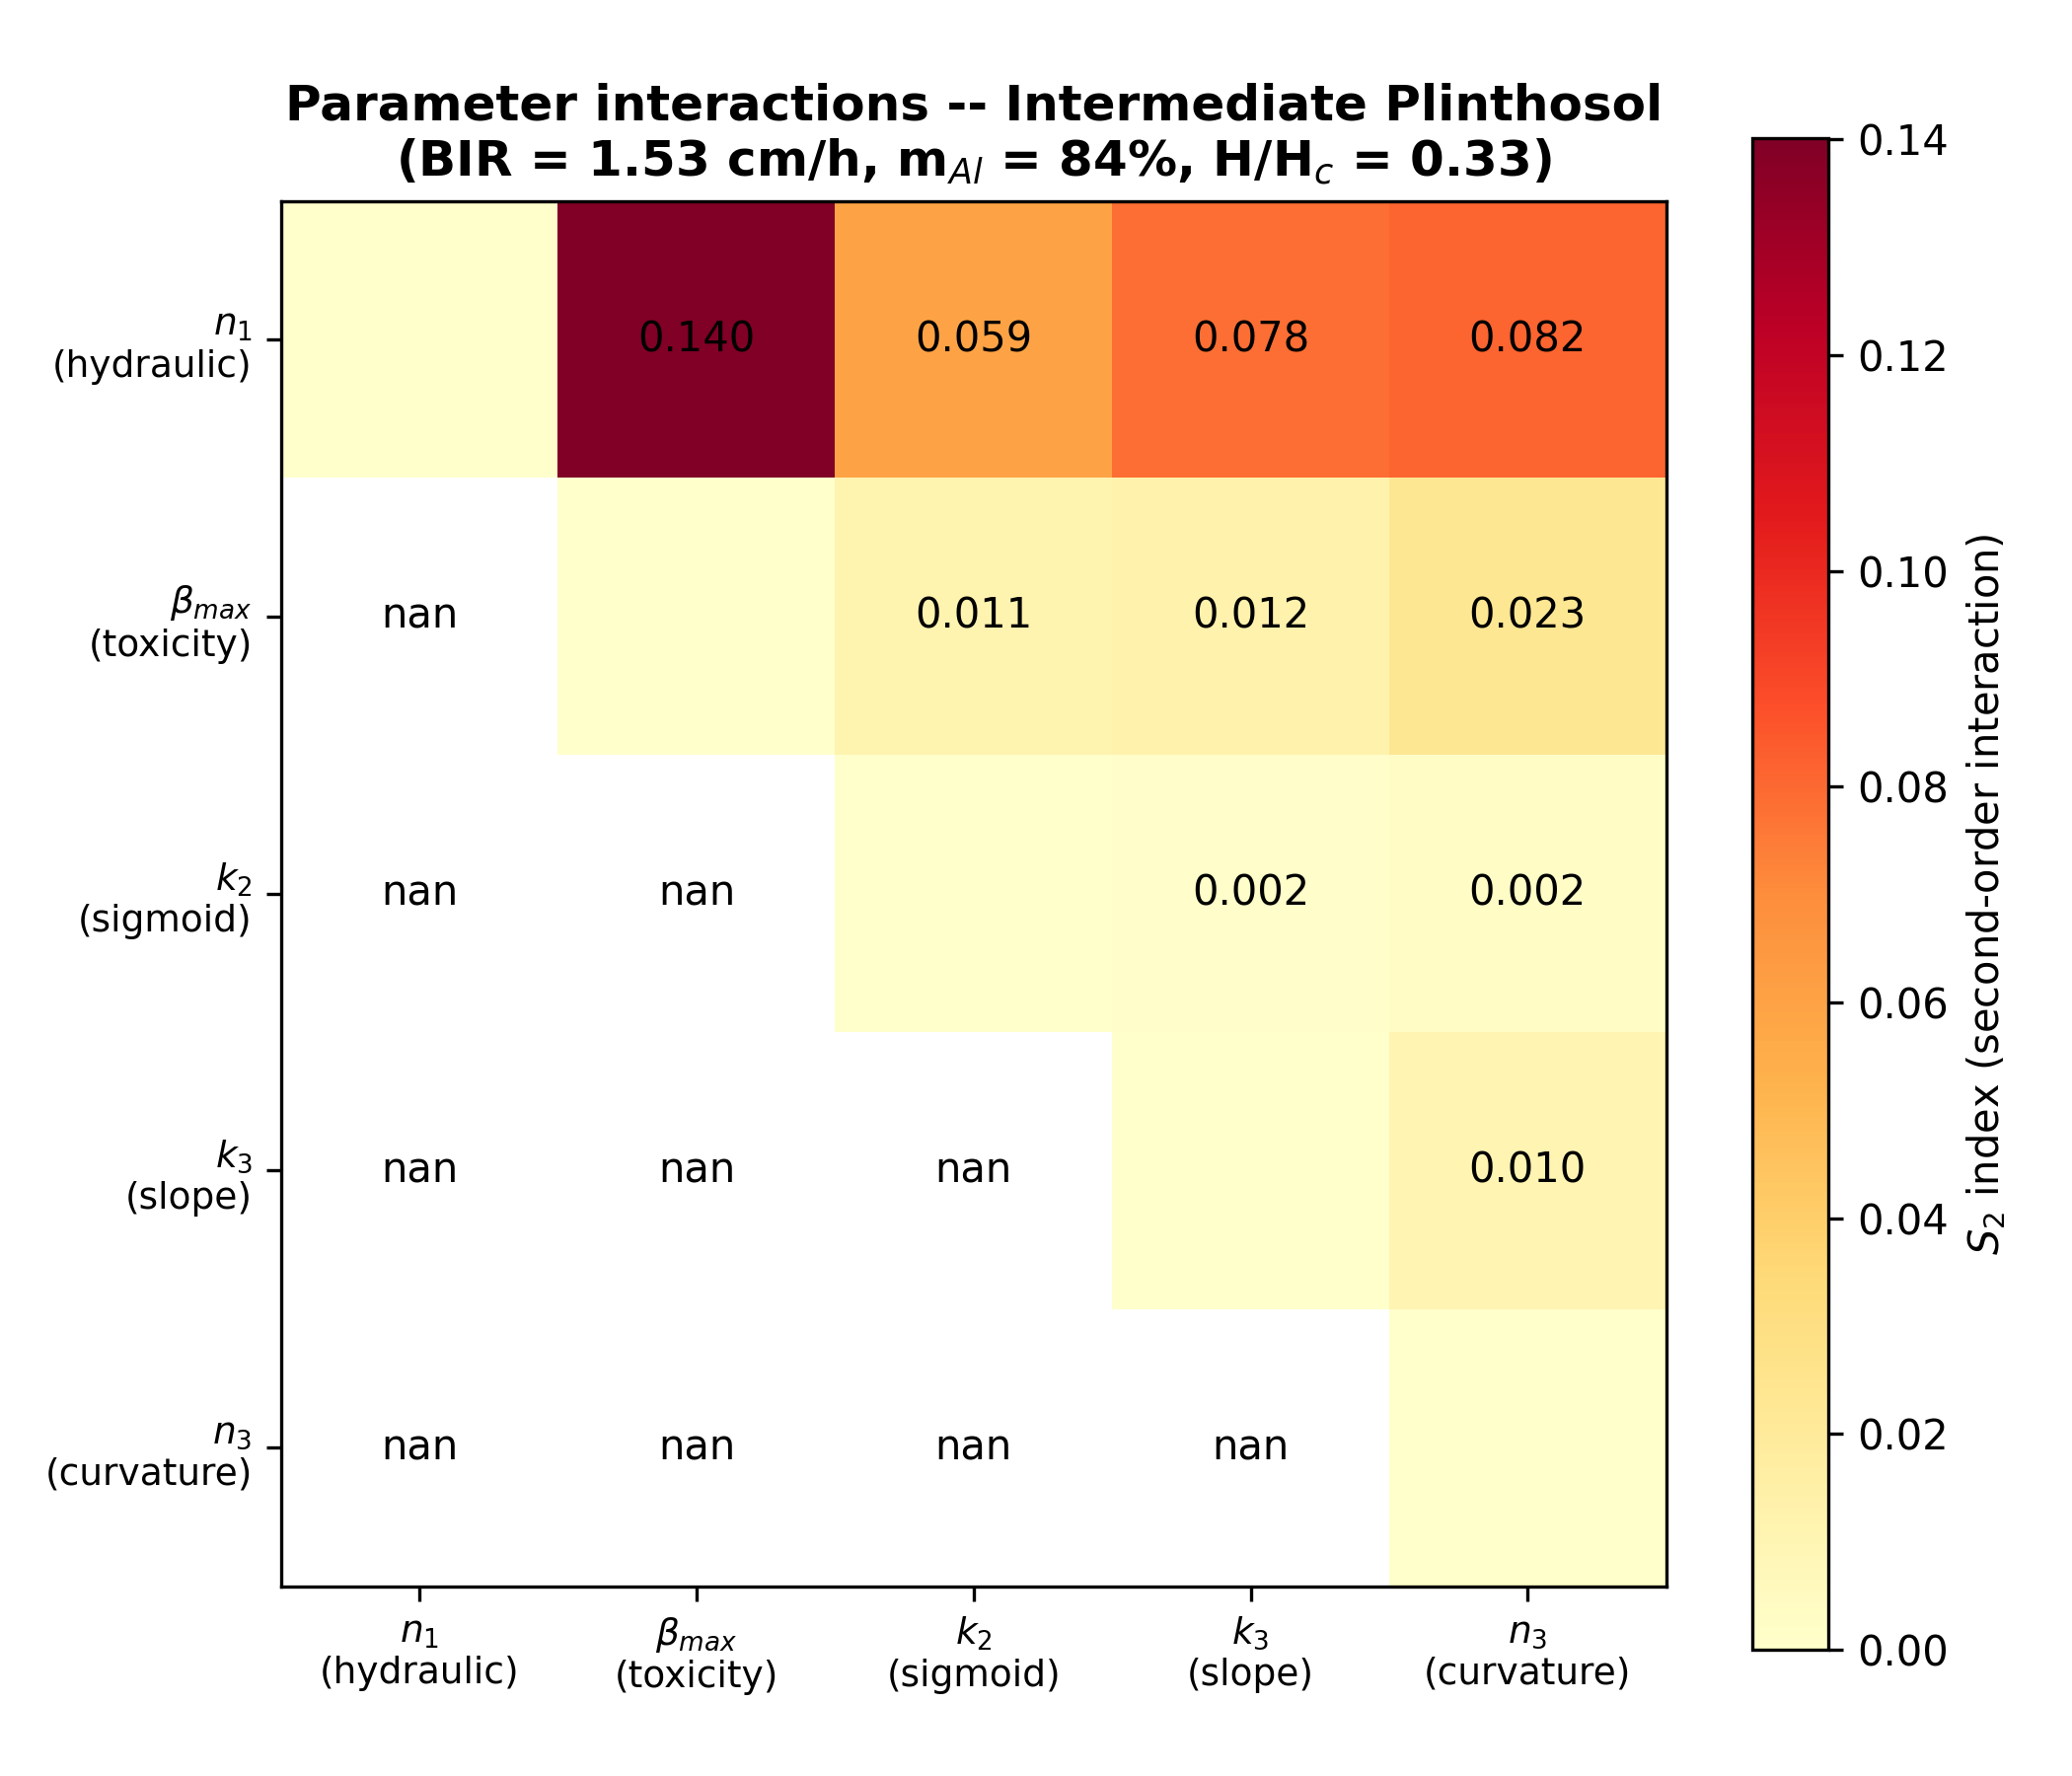
\includegraphics[width=0.7\textwidth]{fig_04_interacoes_s2.png}
\caption{Sobol second-order interaction matrix ($S_2$) for the intermediate Plinthosol scenario ($\mathrm{BIR} = 1.53$~cm/h, aluminum saturation $= 84\%$, $H/H_c = 0.33$).}
\label{fig:interacoes}
\end{figure}

\subsection{Geotechnical validation of $\gamma$ (Test~3)}

The fit of $\gamma = 1 + k_3(H/H_c)^{n_3}$ to the Rankine-derived proxy $\delta_{\mathrm{geo}}$ converged to $k_3 = 6.50$ and $n_3 = 4.51$ (Fig.~\ref{fig:taludes}), parameterising the geotechnical term required by the extended RUSLE in gullies where collapse adds to hydraulic detachment, values substantially higher than the synthetic-calibration targets ($3.0$ and $2.0$). The divergence is physically coherent because the volumetric contribution of collapse grows more rapidly with $H/H_c$ than the originally proposed quadratic expansion, owing to the cubic or quartic dependence of wedge volume on wall height \citep{fredlund_rahardjo_1993}. The exponent $n_3 \approx 4.5$ implies that $\gamma$ remains negligible for $H/H_c < 0.3$ and rises abruptly above this threshold, consistent with the field observation that only F4 ($H/H_c = 0.42$) and F5 (0.45) were classified as incipient gullies by the fuzzy system.

In gullies on Barreiras Group sediments in Bananal (SP), \citet{oliveira_1991} identified analogous behavior, with the transition between concentrated-flow erosion and mass failure occurring above $H/H_c \approx 0.35$--0.40. In southeastern Spain, \citet{vandekerckhove_et_al_2003} quantified headcut retreat rates of 0.01--0.89~m/yr, with the highest values in features with vertical walls and depth exceeding 1.5~m, a condition in which gravitational instability surpasses hydraulic detachment. In a retreat model validated for high $H/H_c$ ratios, \citet{campo_bescos_et_al_2013} corroborated this relationship by identifying a collapse component exceeding the hydraulic, supporting the pronounced non-linearity ($n_3 > 4$) observed here.

\begin{figure}[htbp]
\centering
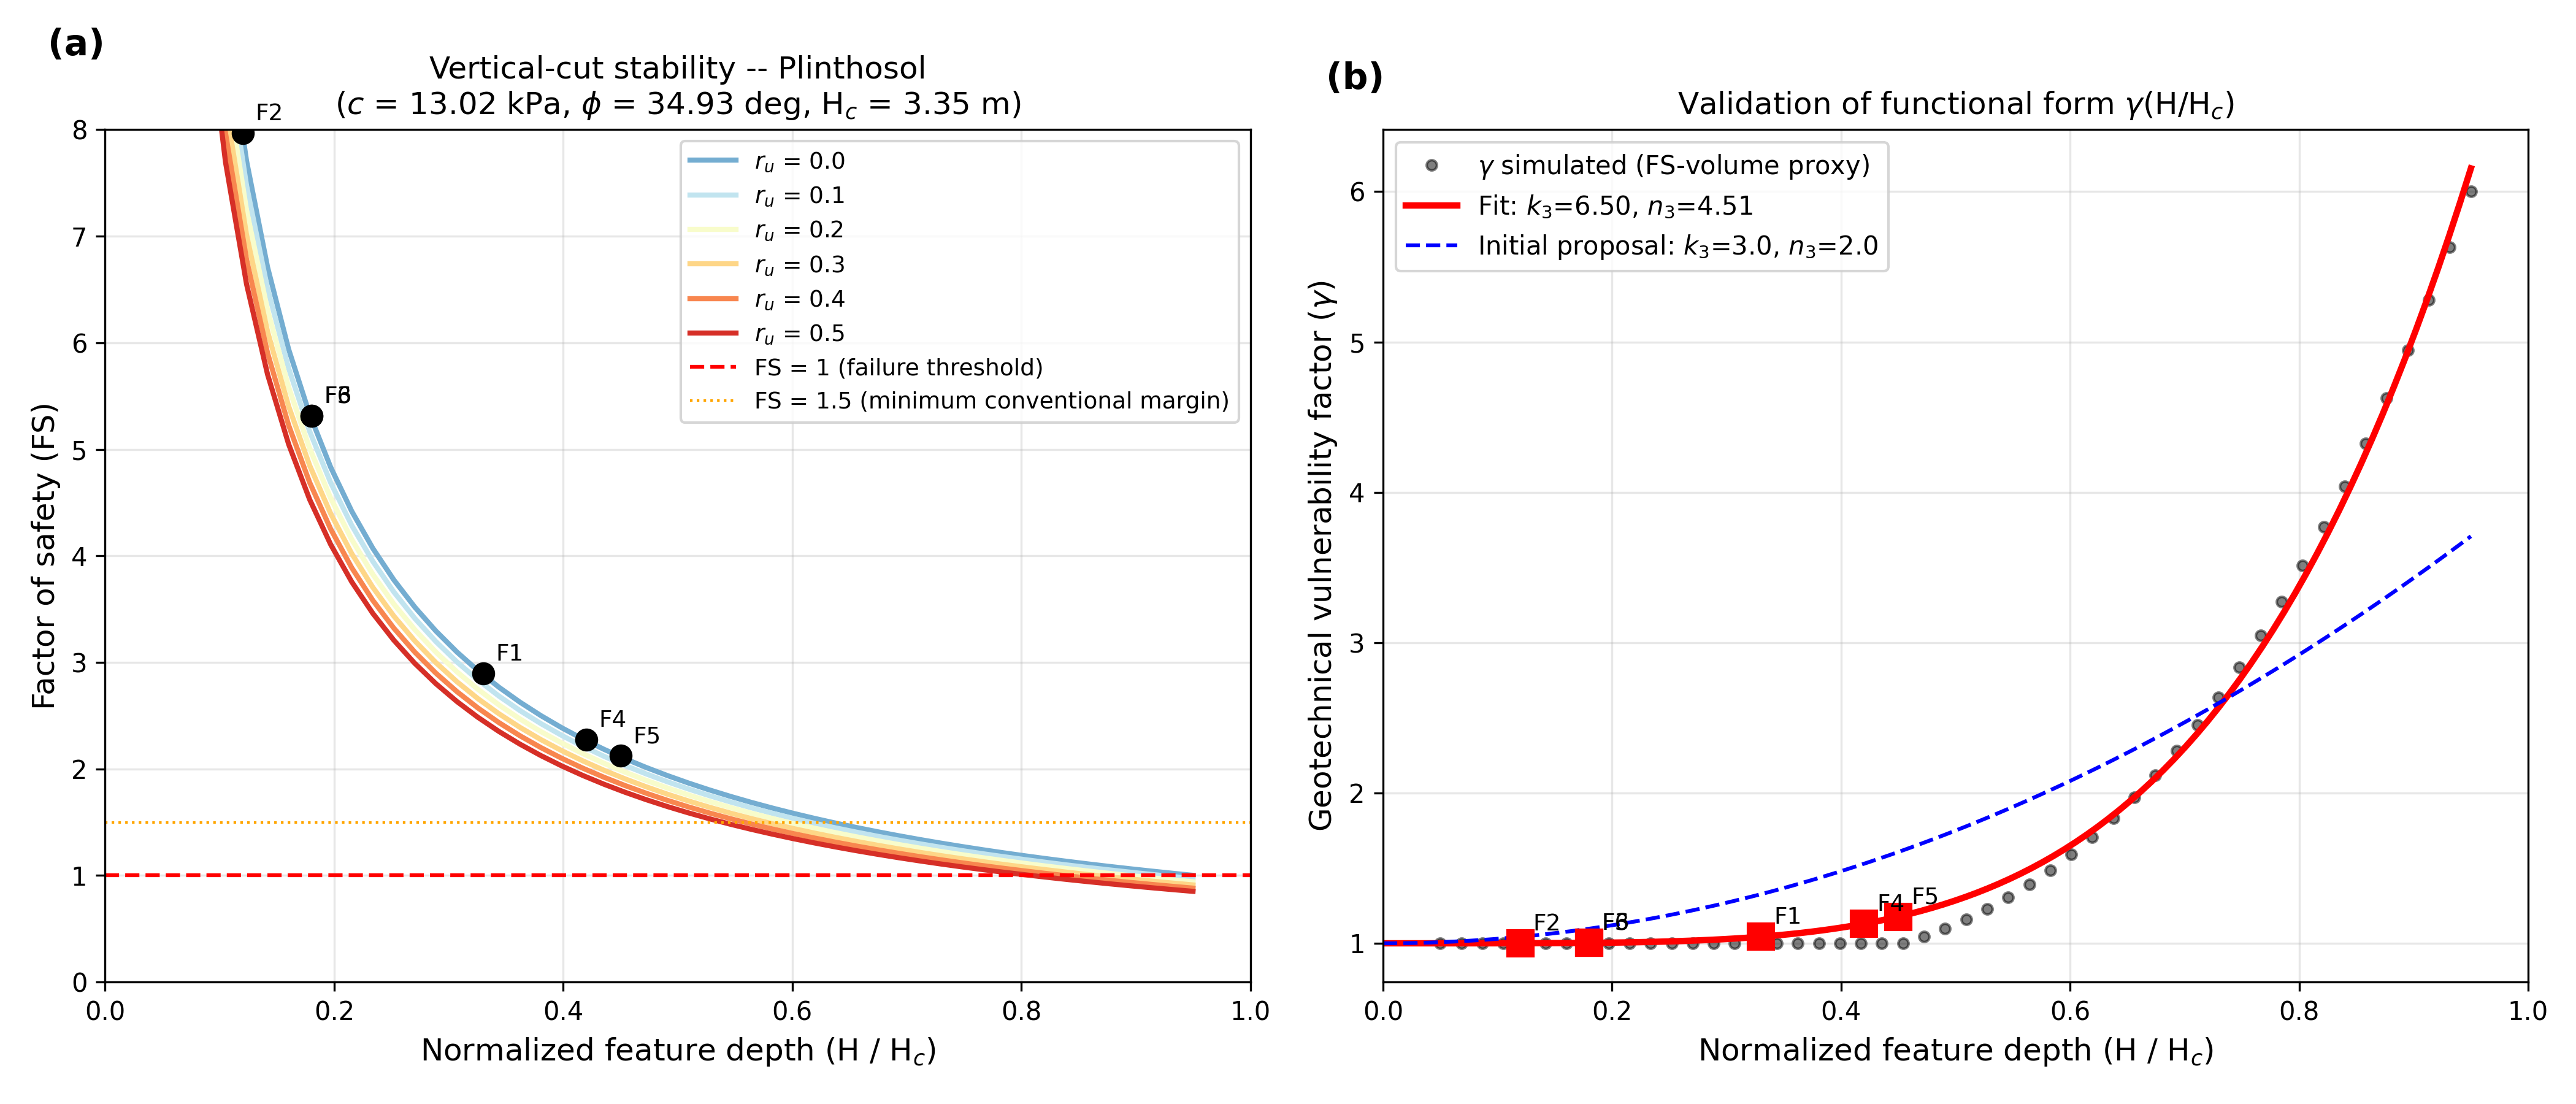
\includegraphics[width=\textwidth]{fig_05_estabilidade_taludes.png}
\caption{(a)~Rankine factor of safety (FS) as a function of $H/H_c$ under different relative pore pressures ($r_u$). (b)~Proxy $\delta_{\mathrm{geo}}$ and power fit $\gamma = 1 + 6.50 \times (H/H_c)^{4.51}$. Red dots: real features F1--F6.}
\label{fig:taludes}
\end{figure}

The factor of safety is sensitive to relative pore pressure, decreasing from 2.12 to 1.93 in F5 when $r_u$ increases from 0 to 0.3. Under prolonged saturation during extreme rainfall, this reduction may bring FS close to unity and trigger lateral collapses that feedback soil loss, a mechanism that \citet{vanmaercke_et_al_2021} identified as responsible for up to 60\% of volumetric gully advance in subtropical regions. RUSLE corrected by the $\gamma$ term accommodates this process without requiring a dynamic stability model.

All six real features exhibited FS $>$\,2.0 for $r_u = 0$ and FS $>$\,1.8 for $r_u = 0.3$ (Table~\ref{tab:fs}), a margin consistent with classification as gullies without active collapse according to \citet{poesen_2018}. The fitted $\gamma$ for F5 ($H/H_c = 0.45$) reached 1.18, indicating 18\% geotechnical amplification over basal erodibility, while F2 ($H/H_c = 0.12$) remains at $\gamma = 1.00$. For features with $H/H_c > 0.6$, documented in regional gullies, $\gamma$ may exceed 2.0, a condition in which the geotechnical mechanism would contribute with magnitude comparable to or exceeding the hydraulic and phytotoxic amplifications and would justify the mandatory inclusion of the term in regional RUSLE applications.

\begin{table}[htbp]
\centering
\caption{Factor of safety and fitted $\gamma$ for the six real erosion features.}
\label{tab:fs}
\small
\begin{tabular}{@{}c r r r r r@{}}
\toprule
Feature & $H$ (m) & $H/H_c$ & FS ($r_u = 0$) & FS ($r_u = 0.3$) & $\gamma$ fitted \\
\midrule
F1 & 1.10 & 0.33 & 2.90 & 2.64 & 1.04 \\
F2 & 0.40 & 0.12 & 7.97 & 7.25 & 1.00 \\
F3 & 0.60 & 0.18 & 5.31 & 4.83 & 1.00 \\
F4 & 1.40 & 0.42 & 2.28 & 2.07 & 1.13 \\
F5 & 1.50 & 0.45 & 2.12 & 1.93 & 1.18 \\
F6 & 0.60 & 0.18 & 5.31 & 4.83 & 1.00 \\
\bottomrule
\end{tabular}
\end{table}

\subsection{Runoff generation and $\alpha$ validation (Test~4)}

The Plinthosol ($K_{\mathrm{sat,eff}} = 0.50$~cm/h, limiting BAc) generated, under the Green--Ampt model, a runoff coefficient of 0.20 for $I_{30} = 30$~mm/h and 0.56 for $I_{30} = 60$~mm/h (Fig.~\ref{fig:infiltracao}a), reflecting the subsurface impedance that converts the non-infiltrated fraction to Hortonian runoff even under moderate intensities. Adopting the limiting-horizon $K_{\mathrm{sat}}$ as the effective conductivity follows \citet{wang_et_al_1999}, in which the least-permeable layer controls time to ponding independently of the upper-layer conductivity, a premise suitable for Plinthosols whose plinthic horizon has conductivity one to two orders of magnitude below that of the A horizon. The Acrisol ($K_{\mathrm{sat,eff}} = 1.0$~cm/h) yielded RC = 0.37 for $I_{30} = 60$~mm/h, intermediate between the two extremes and consistent with the partial impedance of the plinthite-free Bt horizon.

\begin{figure}[htbp]
\centering

\includegraphics[width=\textwidth]{fig_06_infiltracao_escoamento.png}
\caption{(a)~Runoff coefficient (RC) as a function of $I_{30}$ for the three soil profiles (Green--Ampt, 60-min event). (b)~RC/RC$_{\mathrm{Fer}}$ ratio compared with theoretical $\alpha$ (Eq.~\ref{eq:alpha}) for three values of $n_1$.}
\label{fig:infiltracao}
\end{figure}

The Ferralsol ($K_{\mathrm{sat,eff}} = 8.0$~cm/h) generated no surface runoff at any tested intensity (RC = 0 for $I_{30}$ up to 100~mm/h), indicating that the threshold $\mathrm{BIR_{ref}} = 6$~cm/h is conservative and that soils with effective $K_{\mathrm{sat}}$ exceeding this level tend to operate fully in an infiltration-dominated regime. The RC of 0.56 obtained for the Plinthosol is compatible with the magnitude expected in soils whose limiting horizon has $K_{\mathrm{sat}}$ below 1~cm/h \citep{morgan_2005}, while the absence of runoff in the Ferralsol is coherent with deep, well-drained soils \citep{bertoni_lombardi_neto_2017}. The differentiation supports the use of the Ferralsol as a negative control where $K_{\mathrm{obs}} \approx K_{\mathrm{RUSLE}}$ and dispenses with correction.

The hydrograph under $I_{30} = 60$~mm/h (Fig.~\ref{fig:hidrograma}) illustrates the temporal difference in runoff generation, with the Plinthosol reaching steady state in less than 10~min and the Acrisol requiring approximately 25~min, reflecting the inverse proportion between $K_{\mathrm{sat,eff}}$ and the time to ponding predicted by infiltration-excess theory \citep{horton_1933}. The absence of Ferralsol runoff throughout the 60-min event is coherent with soils whose effective $K_{\mathrm{sat}}$ exceeds any probable rainfall intensity at the study site.

The temporal contrast has practical implications for the dimensioning of erosion-control structures associated with the corrected RUSLE. The earlier onset of peak runoff in soils with plinthic horizons suggests that erosive energy reaches high values before dissipative interventions such as permeable check dams can trap upstream sediment, indicating that the $K_{\mathrm{plint}}$ estimate must be combined with a $C \cdot P$ factor specific to low barriers.

\begin{figure}[htbp]
\centering
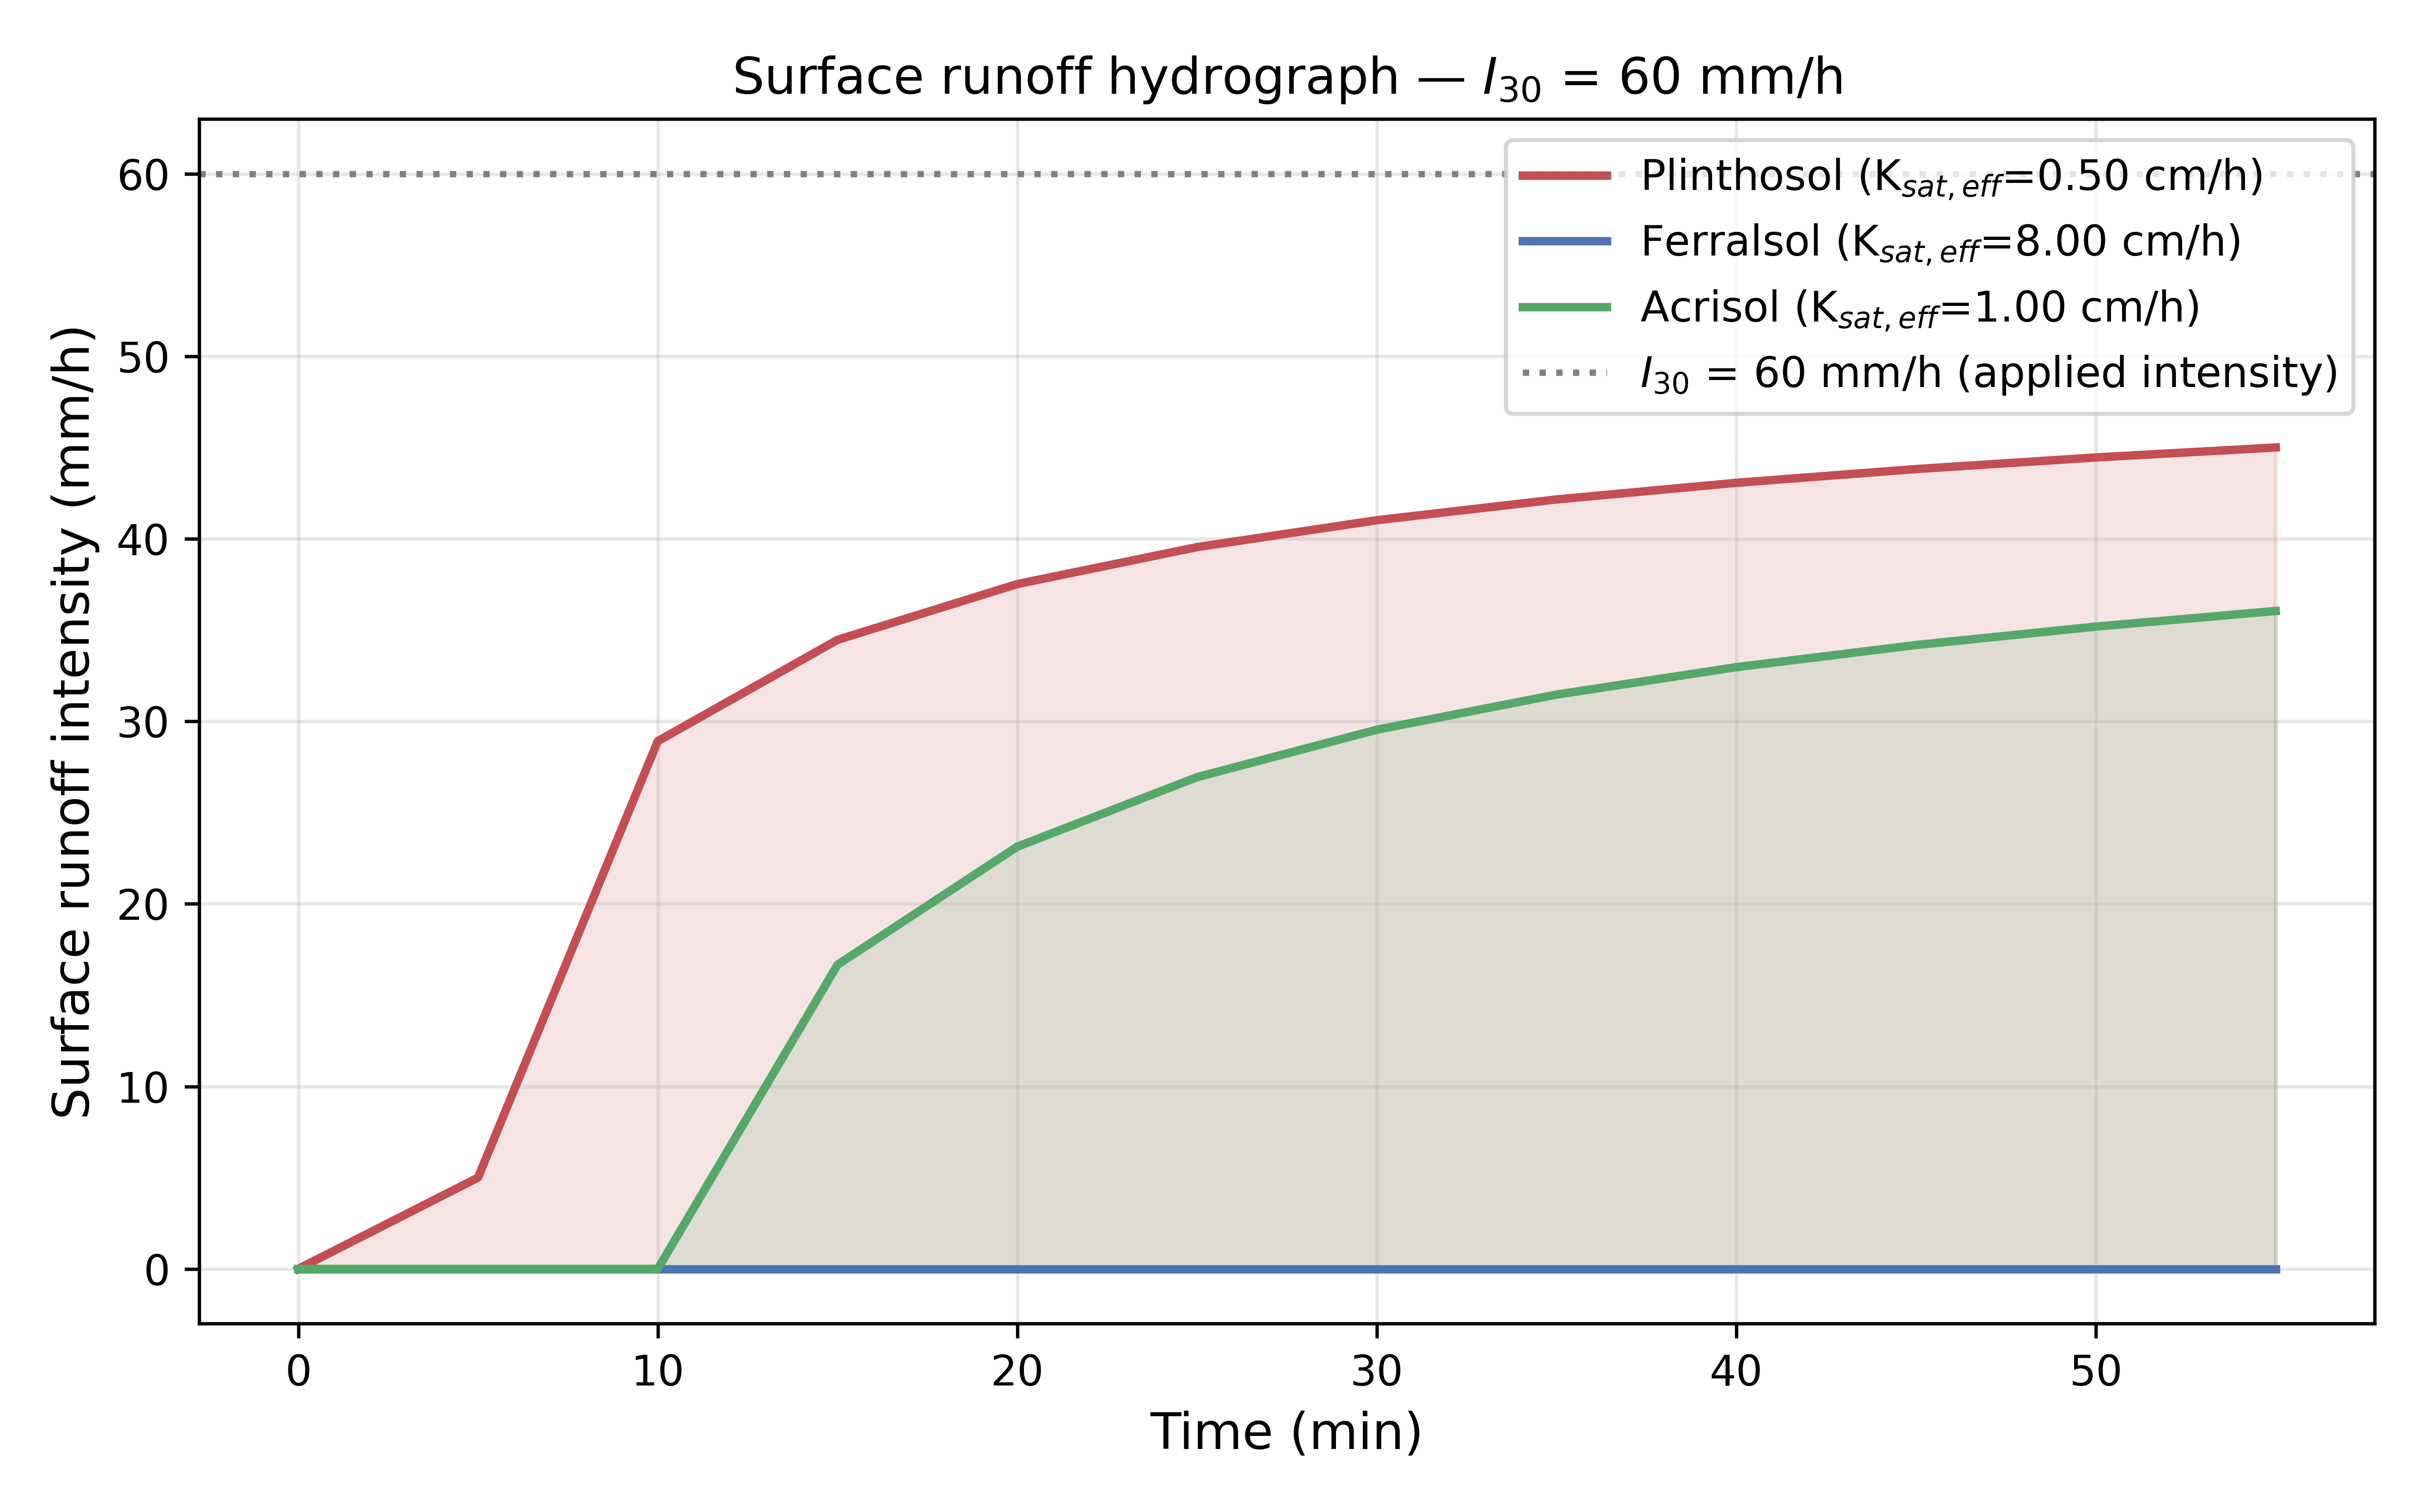
\includegraphics[width=0.8\textwidth]{fig_07_hidrograma_i60.png}
\caption{Surface-runoff hydrograph under $I_{30} = 60$~mm/h for the three soil profiles.}
\label{fig:hidrograma}
\end{figure}

\subsection{Virtual erosion and $\delta$ discrepancy (Test~5)}

The mean discrepancy $\delta_{\mathrm{obs}}$ for the Plinthosol ($2.71 \pm 0.91$ for $I_{30} \geq 40$~mm/h) fell below the $\delta_{\mathrm{mod}} = 8.01$ predicted with the target parameters, yielding a relative error of 66\% (Fig.~\ref{fig:erosao}c--d) and gauging the magnitude of calibration still required for RUSLE with $K_{\mathrm{plint}}$ to approach the erosive response simulated by a physical detachment model.

The overestimation is expected because the ``true'' parameters ($n_1 = 1.0$, $\beta_{\max} = 2.5$ etc.) were set within plausible ranges and do not represent the actual site. The same trend manifests in the Acrisol ($\delta_{\mathrm{obs}} = 0.61$ only for $I_{30} = 100$~mm/h, versus $\delta_{\mathrm{mod}} = 2.29$), while the absence of erosion in the Ferralsol ($\delta_{\mathrm{obs}}$ indeterminate due to zero numerator) is consistent with $\delta \approx 1$ predicted by the model, reinforcing the pedological specificity of the correction factor.

A second source of discrepancy lies in the detachment model ($D = k_r(\tau - \tau_c)$), which does not incorporate transport-capacity limitation and may underestimate $K_{\mathrm{obs}}$ in extreme events in which sediment is exported from the plot before accumulating. In WEPP simulations, \citet{nearing_nicks_1998} identified analogous behavior, with predicted erosion exceeding measured erosion in high-intensity events when transport capacity was not imposed as a limiter. In soils with high dispersible-clay fractions, a category that includes Plinthosols owing to kaolinite presence and low subsurface structural stability, \citet{deviren_saygin_et_al_2018} demonstrated that process-based detachment erodibility diverges from empirical USLE erodibility.

\begin{figure}[htbp]
\centering
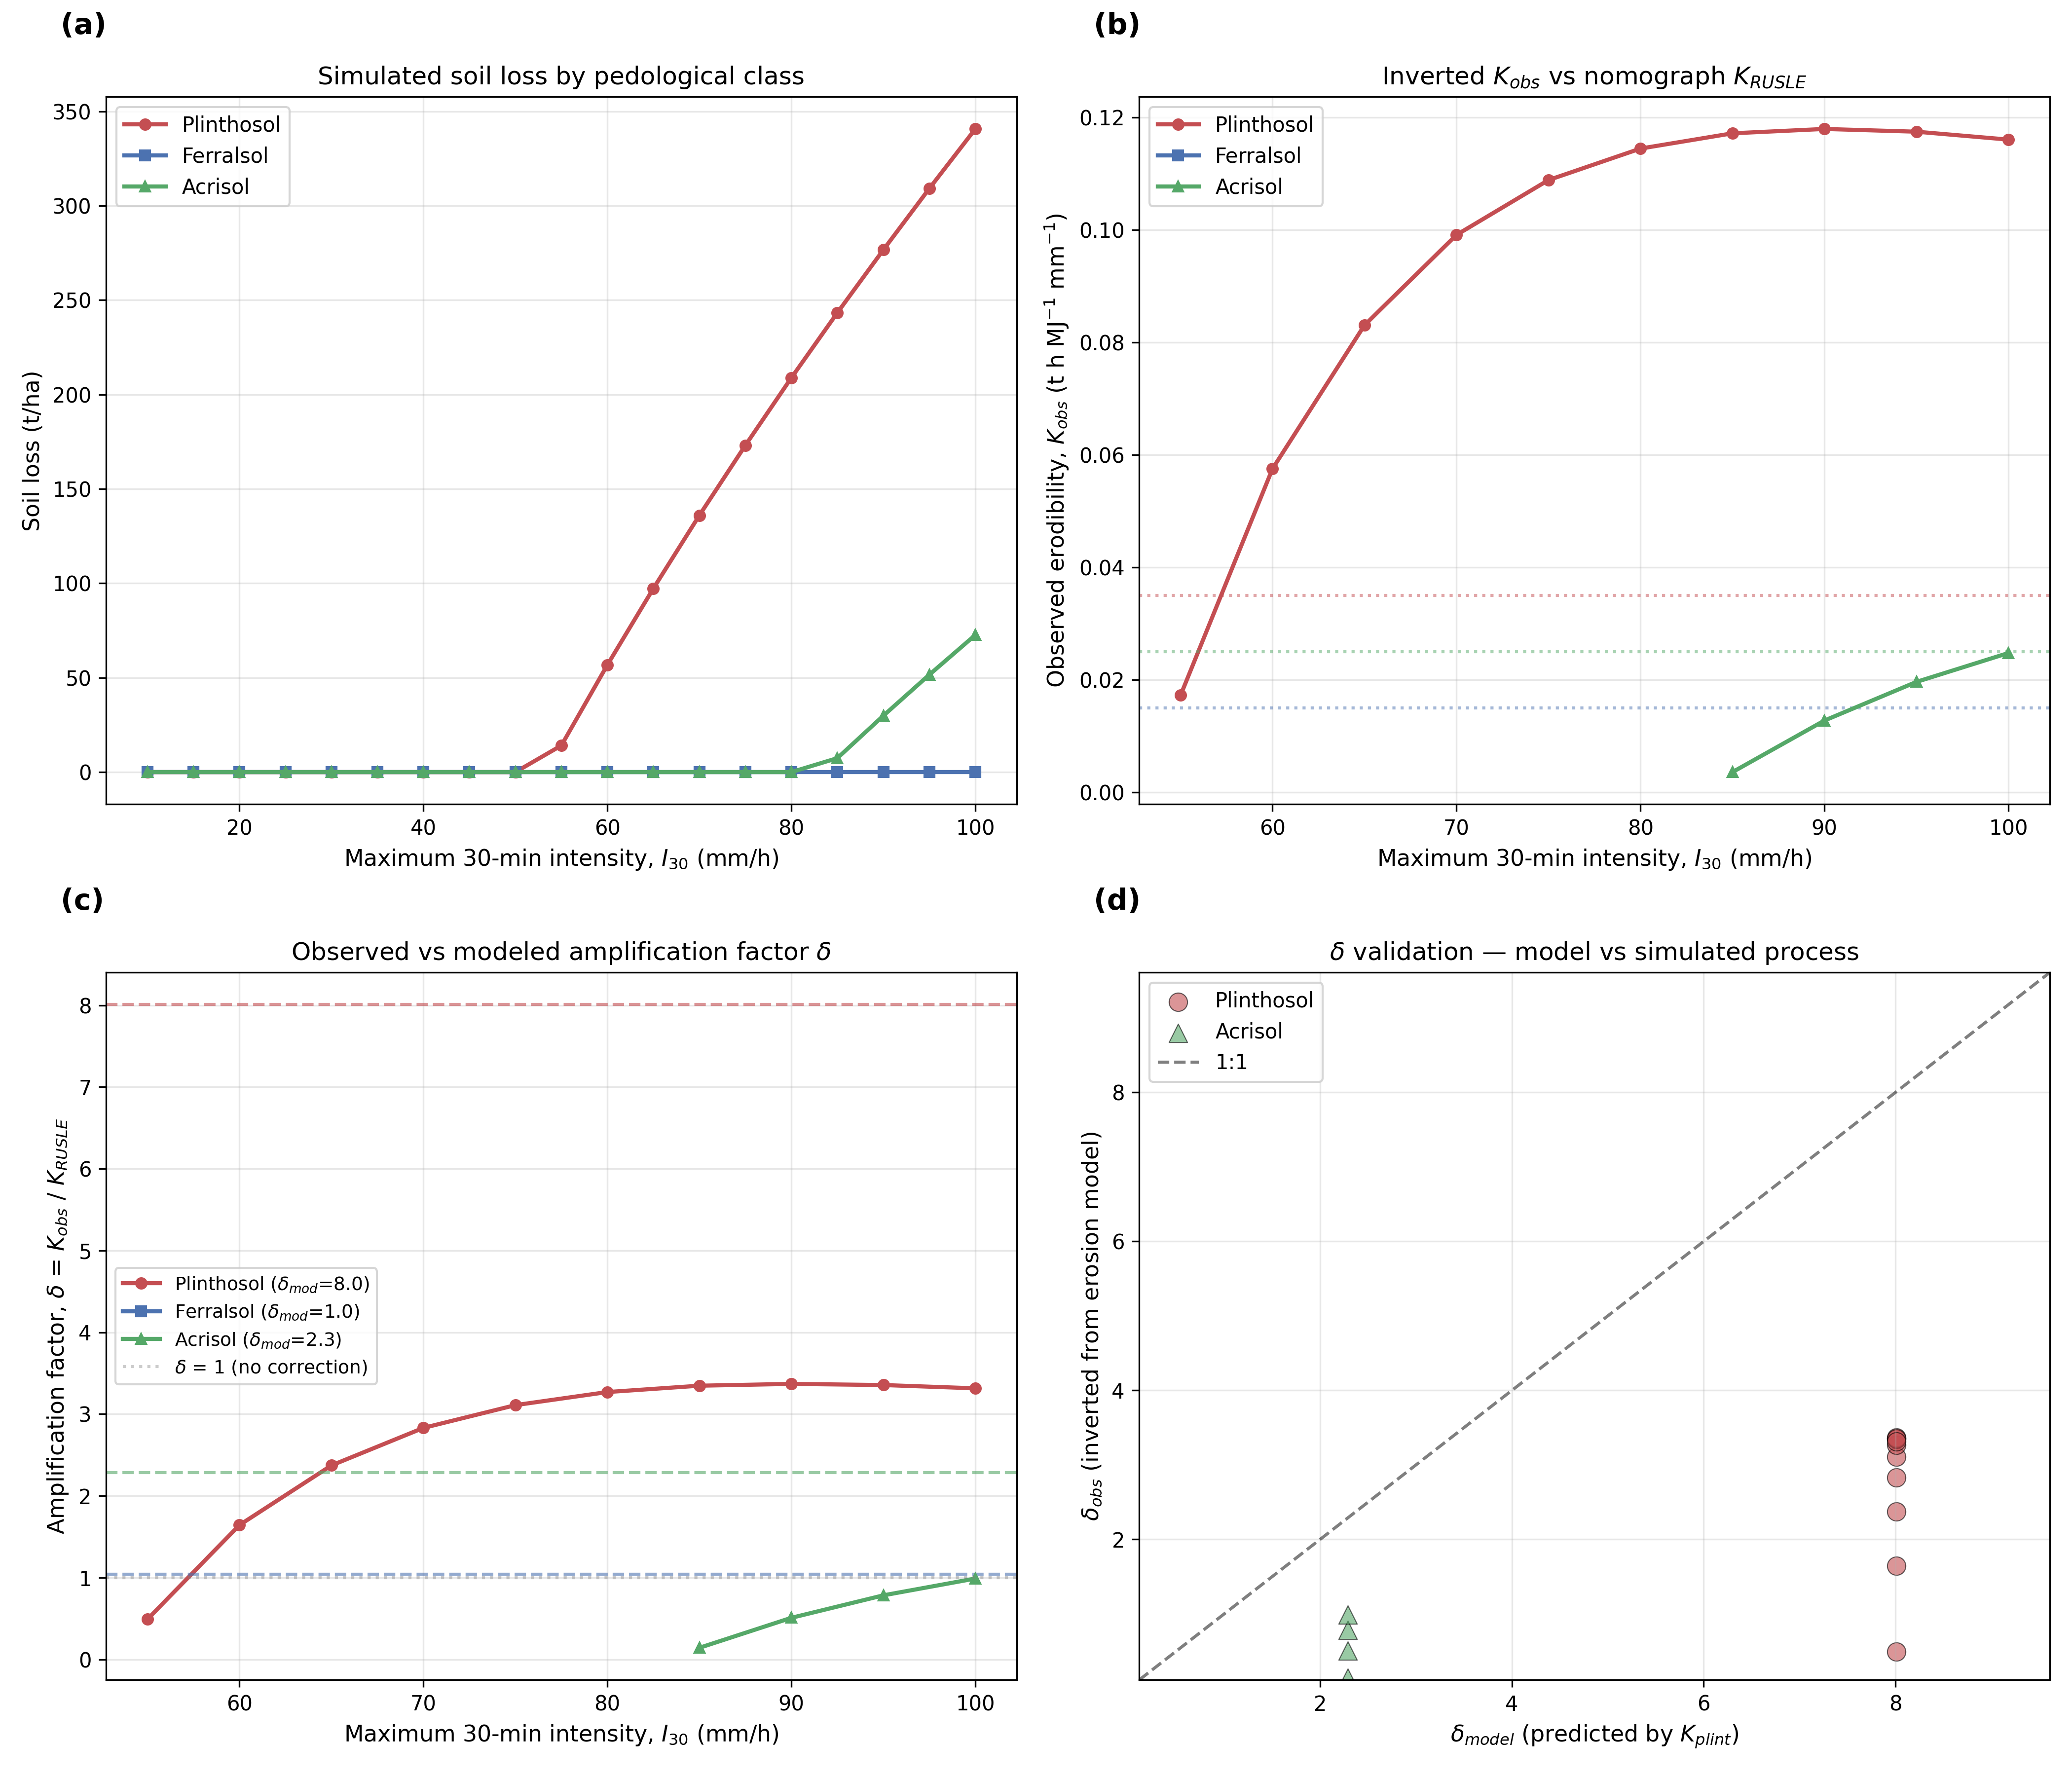
\includegraphics[width=\textwidth]{fig_08_erosao_virtual.png}
\caption{(a)~Soil loss by pedological class and $I_{30}$. (b)~$K_{\mathrm{obs}}$ compared with $K_{\mathrm{RUSLE}}$ (dotted lines). (c)~$\delta_{\mathrm{obs}} = K_{\mathrm{obs}}/K_{\mathrm{RUSLE}}$ versus $I_{30}$, with $\delta_{\mathrm{mod}}$ as reference (dashed). (d)~Validation $\delta_{\mathrm{obs}}$ versus $\delta_{\mathrm{mod}}$ (1:1 line).}
\label{fig:erosao}
\end{figure}

Despite the parametric overestimation, $K_{\mathrm{plint}}$ preserves the pedological hierarchy (Plinthosol $>$ Acrisol $>$ Ferralsol) and generates $\delta$ values structurally consistent with the simulated processes, a result coherent with the premise that the multiplicative structure captures the relative contribution of each amplifying mechanism even when absolute parameter values are uncalibrated \citep{renard_et_al_1997}. The $K_{\mathrm{obs}}$ values of 0.058--0.116~t\,h\,MJ$^{-1}$\,mm$^{-1}$ obtained for the Plinthosol lie in the upper range documented for Brazilian soils with limiting subsurface horizons \citep{lafayette_cantalice_coutinho_2011,cassol_et_al_2023} and exceed the original nomograph estimates by 2--8 times \citep{wischmeier_et_al_1971}.

The systematic underestimation of the RUSLE nomograph in tropical soils with dominant subsurface processes was reported by \citet{alewell_et_al_2019}, and \citet{torri_poesen_2014} had already indicated that erodibility is an emergent property of the profile rather than solely of the surface horizon. This framework supports the need for correction factors integrating pedological information at depth, a task that $K_{\mathrm{plint}}$ executes with five parameters and three field variables.

On plots in Sicily, \citet{bagarello_et_al_2012} measured 0.040--0.090~t\,h\,MJ$^{-1}$\,mm$^{-1}$ in soils with a subsurface clay horizon, a range compatible with that obtained here despite the climatic contrast because textural discontinuity generates comparable hydraulic impedance in both contexts. In calcareous soils with subsurface impedance in Iran, \citet{ostovari_et_al_2016} reported analogous underestimation, and in southern Bahia \citet{francois_et_al_2024} identified $K$ as the most sensitive RUSLE parameter. The convergence across contrasting geomorphological provinces suggests that $K_{\mathrm{plint}}$ may have applicability beyond Plinthosols, extending to soils whose subsurface horizon governs the hydrological response.

Field calibration with data from plots under natural rainfall can adjust the five parameters to minimize the distance between $\delta_{\mathrm{obs}}$ and $\delta_{\mathrm{mod}}$. The Green--Ampt model assumes a homogeneous wetting front and a single effective $K_{\mathrm{sat}}$, and the antecedent moisture deficit ($\theta_s - \theta_i$) and the retention curve introduce additional uncertainty that may affect the absolute magnitude of predicted runoff and, therefore, $\delta_{\mathrm{obs}}$. A Bayesian framework incorporating Rankine geotechnical priors and retention-curve uncertainty may mitigate both the residual equifinality of $k_3$/$n_3$ and the sensitivity to Green--Ampt assumptions \citep{beven_freer_2001}.

\subsection{Observational noise envelope and cover-management prior from an exploratory field campaign}
\label{sec:empirical-anchor}

The variability observed on the Plinthosol slope places the calibration of $K_{\mathrm{plint}}$ in a more heterogeneous regime than that represented by the synthetic noise in Test~1. The bare-soil plots and the plots with low stone palisades were monitored across fifteen sediment collections between 13 May and 24 November 2025. Cumulative rainfall extracted from the 21-year daily series of the project climatological station (less than 500~m from the ramps) reached 846.6~mm, equivalent to 77.5\% of the 1092~mm historical annual mean and corresponding to an estimated $EI_{30}$ of 2944.7~MJ\,mm\,ha$^{-1}$\,h$^{-1}$, about 78\% of the 3799~MJ\,mm\,ha$^{-1}$\,h$^{-1}$\,yr$^{-1}$ regional mean. Mean cumulative sediment yield was 2396.3~g per bare-soil ramp and 1024.4~g per low-stone-palisade ramp, equivalent to 19.97 and 8.54~t\,ha$^{-1}$ respectively over the monitored interval. The coefficient of variation among the seven bare-soil replicates averaged $\sim$80\%, a value compatible with the dispersion documented by \citet{nearing_govers_norton_1999} in replicated erosion plots, where small differences in microtopography, initial cover and flow connectivity increase the variance of soil loss even under nominally identical treatment.

This variability does not invalidate the recoverability demonstrated in Test~1, but it indicates that field calibration is likely to require hierarchical models capable of separating measurement error, between-ramp heterogeneity and event-specific response. The bare-soil to palisade sediment ratio of 2.34 indicates reduced sediment mobilization by a fixed permeable barrier under identical rainfall and soil conditions, a mechanism consistent with evaluations of stone bunds in northern Ethiopia, where transverse structures reduced hydro-sedimentary connectivity by retaining sediment upslope and shortening the effective slope length \citep{nyssen_et_al_2007}. The response of these barriers, however, varies with hillslope position, sediment redistribution and local soil properties, as observed by \citet{vancampenhout_et_al_2006}, so the ratio of 2.34 does not represent a universal palisade efficiency but a local prior of $C \cdot P \approx 0.43$ for the joint estimation of $K_{\mathrm{plint}} \cdot C \cdot P$ in the instrumented Wischmeier plots. Because the $K_{\mathrm{plint}}$ model operates with $C = P = 1$ by definition, this prior prevents a sediment reduction produced by cover-management from being attributed to intrinsic erodibility.

\begin{table}[htbp]
\centering
\caption{Observational constraints derived from the exploratory field campaign and their implications for the statistical design of the $K_{\mathrm{plint}}$ calibration phase.}
\label{tab:comparativa}
\small
\begin{tabular}{@{}l c c@{}}
\toprule
Empirical constraint & Observed value & Implication for calibration design \\
\midrule
Bare-soil inter-replicate CV & $\sim$80\% & Bayesian hierarchical models preferred over pooled regression \\
Bare-soil : stone-palisade sediment ratio & 2.34 & $C \cdot P \approx 0.43$ prior for combined $K_{\mathrm{plint}} \cdot C \cdot P$ estimation \\
Cumulative rainfall in interval & 846.6~mm (78\% of annual $EI_{30}$) & Single-station pluviograph sufficient for $R$-factor estimation \\
Ramp length & 2.40~m & Full Wischmeier length (22.13~m) required for unbiased $K_{\mathrm{obs}}$ \\
Runoff gauging & Absent & Geib dividers + storage tanks required for runoff partitioning \\
$EI_{30}$ computation & Scaled by interval $P$ & Per-event tipping-bucket record required \\
\bottomrule
\end{tabular}
\end{table}

The geometric and instrumental limitations of the exploratory arrangement, especially the ramp length one order of magnitude below the Wischmeier standard, the absence of runoff measurement and the $EI_{30}$ scaled by interval rainfall rather than computed for isolated events, restrict the direct use of these data to estimate unbiased $K_{\mathrm{obs}}$, but do not compromise the role of the campaign as a source of observational constraints for the five computational tests (Table~\ref{tab:comparativa}). The noise envelope of $\sim$80\% delimits the range in which the parameter recoverability demonstrated in Test~1 remains useful for field calibration, whereas the bare-soil/palisade ratio of 2.34 empirically quantifies the cover-management factor associated with fixed permeable barriers under the same hydro-sedimentary regime in which $K_{\mathrm{plint}}$ was formulated. Together, the five computational tests and the constraints derived from the exploratory campaign support that the proposed multiplicative structure is mathematically identifiable, physically coherent with the tropical pedological gradient and empirically compatible with the field variability observed in Plinthosols with active linear erosion, joint conditions that delimit the scope of this study and justify the transition to the subsequent instrumental calibration phase.

%% ================================================================
%%  5. CONCLUSIONS
%% ================================================================
\section{Conclusions}
\label{sec:conclusions}

This study evaluated the parametric identifiability and physical consistency of a five-parameter multiplicative correction of the RUSLE $K$ factor ($K_{\mathrm{plint}}$) for Plinthosols with subsurface hydraulic impedance, through five computational tests anchored in field measurements of a Haplic Plinthosol and in virtual Ferralsol and Acrisol profiles. The proposed formulation reproduced the susceptibility hierarchy among the three pedological classes and preserved the $K_{\mathrm{RUSLE}}$ nomograph as its core, amplifying it only under conditions in which hydraulic impedance, aluminum phytotoxicity and geotechnical vulnerability were simultaneously diagnosed. The hydraulic-biological parameters were recoverable under observational noise, whereas the geotechnical pair exhibited equifinality confined to the shallow normalized-depth range, mitigable by priors derived from Rankine theory. The multiclass design isolated the contribution of each amplifier, with the Ferralsol operating as a negative control, the Acrisol as a partial control and the Plinthosol as a case of convergence among the three mechanisms. The sensitivity analysis indicated dominance of the hydraulic term in the Plinthosol and of the phytotoxic term in the Ferralsol, consistent with the pedological contrast among the classes. The results indicate that the multiplicative correction is mathematically identifiable and physically coherent under the simulated conditions, a necessary condition for the subsequent field-calibration stage. Transfer of the formulation to Acrisols with abrupt textural gradient, Petric Plinthosols and shallow Cambisols constitutes a natural extension, since these classes share analogous pedological discontinuities and tend to require only local recalibration of the five parameters.

%% ================================================================
%%  DECLARATION OF COMPETING INTEREST
%% ================================================================
\section*{Declaration of competing interest}

The authors declare that they have no known competing financial interests or personal relationships that could have appeared to influence the work reported in this paper.

%% ================================================================
%%  ACKNOWLEDGMENTS
%% ================================================================
\section*{Acknowledgments}

The authors thank the Universidade Federal de Sergipe and the Universidade Estadual de Feira de Santana for logistical support, and CAPES for the postdoctoral fellowship.

%% ================================================================
%%  DATA AVAILABILITY
%% ================================================================
\section*{Data availability}

The simulation scripts, input parameters and generated figures are available at Zenodo (\url{https://doi.org/10.5281/zenodo.19483403}). The exploratory slope sediment data and the 21-year daily rainfall series are available in the project repository at \url{https://github.com/ldvsantos/palicada} (directory \texttt{2-DADOS/}).

%% ================================================================
%%  FUNDING
%% ================================================================
\section*{Funding}

This work was supported by CAPES (postdoctoral fellowship).

%% ================================================================
%%  CRediT AUTHOR STATEMENT
%% ================================================================
\section*{CRediT authorship contribution statement}

\textbf{Luiz Diego Vidal Santos:} Conceptualization, Supervision, Project administration, Writing -- review \& editing. \textbf{Emersson Guedes da Silva:} Methodology, Software, Formal analysis, Data curation, Visualization, Writing -- original draft. \textbf{Marcos Oliveira Santos:} Investigation, Data curation. \textbf{Renisson Neponuceno de Ara\'{u}jo Filho:} Investigation, Resources, Writing -- review \& editing. \textbf{Henrique Antonio Silva:} Investigation, Validation. \textbf{J\'{e}misson Mattos dos Santos:} Formal analysis, Writing -- review \& editing.

%% ================================================================
%%  SUPPLEMENTARY MATERIAL
%% ================================================================
\section*{Appendix A. Supplementary material}

Supplementary Material~S1 contains the full derivation of the Rankine critical-height equation used in Section~\ref{sec:test3}.

\bibliographystyle{elsarticle-harv}
\bibliography{referencias_artigos}

\end{document}
